\chapter{Overview of\\Published Work}
\label{chap:PaperOverview}
\textit{This chapter briefly describes the appended papers and developed softwares}
\vfill
\minitoc
\newpage

\section{Paper I}
 This review paper provides a comprehensive overview of studies aiming to advance FRET as a quantitative molecular ruler in studies of nucleic acid structure and dynamics. Although originally intended to be a MiniReview focusing on ensemble techniques we quickly realised during the initial literature search that this topic could not be covered satisfactorily without including single-molecule techniques. The paper includes all aspects of performing quantitative FRET from initial experiment design to data acquisition and analysis and was one of the five most accessed papers from the whole archive of ChemBioChem during September and October 2012.

 \paragraph{Summary of most interesting topics.} The review starts by comparing the advantages and limitations of FRET to those of other structural characterization techniques. Section 2 then provides a short overview of the properties of most popular commercial FRET dyes characterized in nucleic acid environments. Here, Table 1 provides a comprehensive source of references of dye lifetimes, rotational dynamics and interactions with DNA which are all relevant for the design and interpretation of FRET experiments. For many researchers, it may come as a surprise that practically all commercial dyes are somehow influenced by their local environment when positioned in DNA. Section 3 describes the advantages and limitations of alternative FRET probes, including the nucleobase analogues relevant for this thesis.

 Focusing mostly on single-molecule methods, Section 4 describes experimental techniques developed to measure FRET quantitatively. FRET can be measured quantitatively at the single-molecule level both in experiments where the molecules are surface-immobilized and when they are diffusing freely in the solution. However, the quantitative analysis of single-molecule FRET is complex as a result of the low signal-to-noise ratio in such experiments. References to most important papers in this research field is provided in Section 5.

 In order to interpret measured FRET signals into quantitative structural information, the local dynamics of the dyes must be taken into account. Most, if not all, techniques developed to model local probe rotational and diffusional dynamics is described in Section 6 of the paper. These methods include various theoretical models of fluorophore orientational distributions and algorithms optimized for the prediction of dye position and diffusion. In relation to this section, the final section highlights advanced software developed to analyse FRET quantitatively. Most of this software is freely available from the home pages of various group leaders active in this field.

 Section 7 describes recent advanced techniques which exploit FRET to probe three-dimensional nucleic acid structures quantitatively. Most noteworthy is the triangulation-based techniques which exploit the combination of multiple FRET-pair positions in a DNA molecule in order to reconstruct part of the three-dimensional structure.\cite{Muschielok2008,Muschielok2011,Sabir2011,Sabir2012,Wozniak2008,Andrecka2008,Andrecka2009,Balci2011}

\begin{figure}
    \centering
        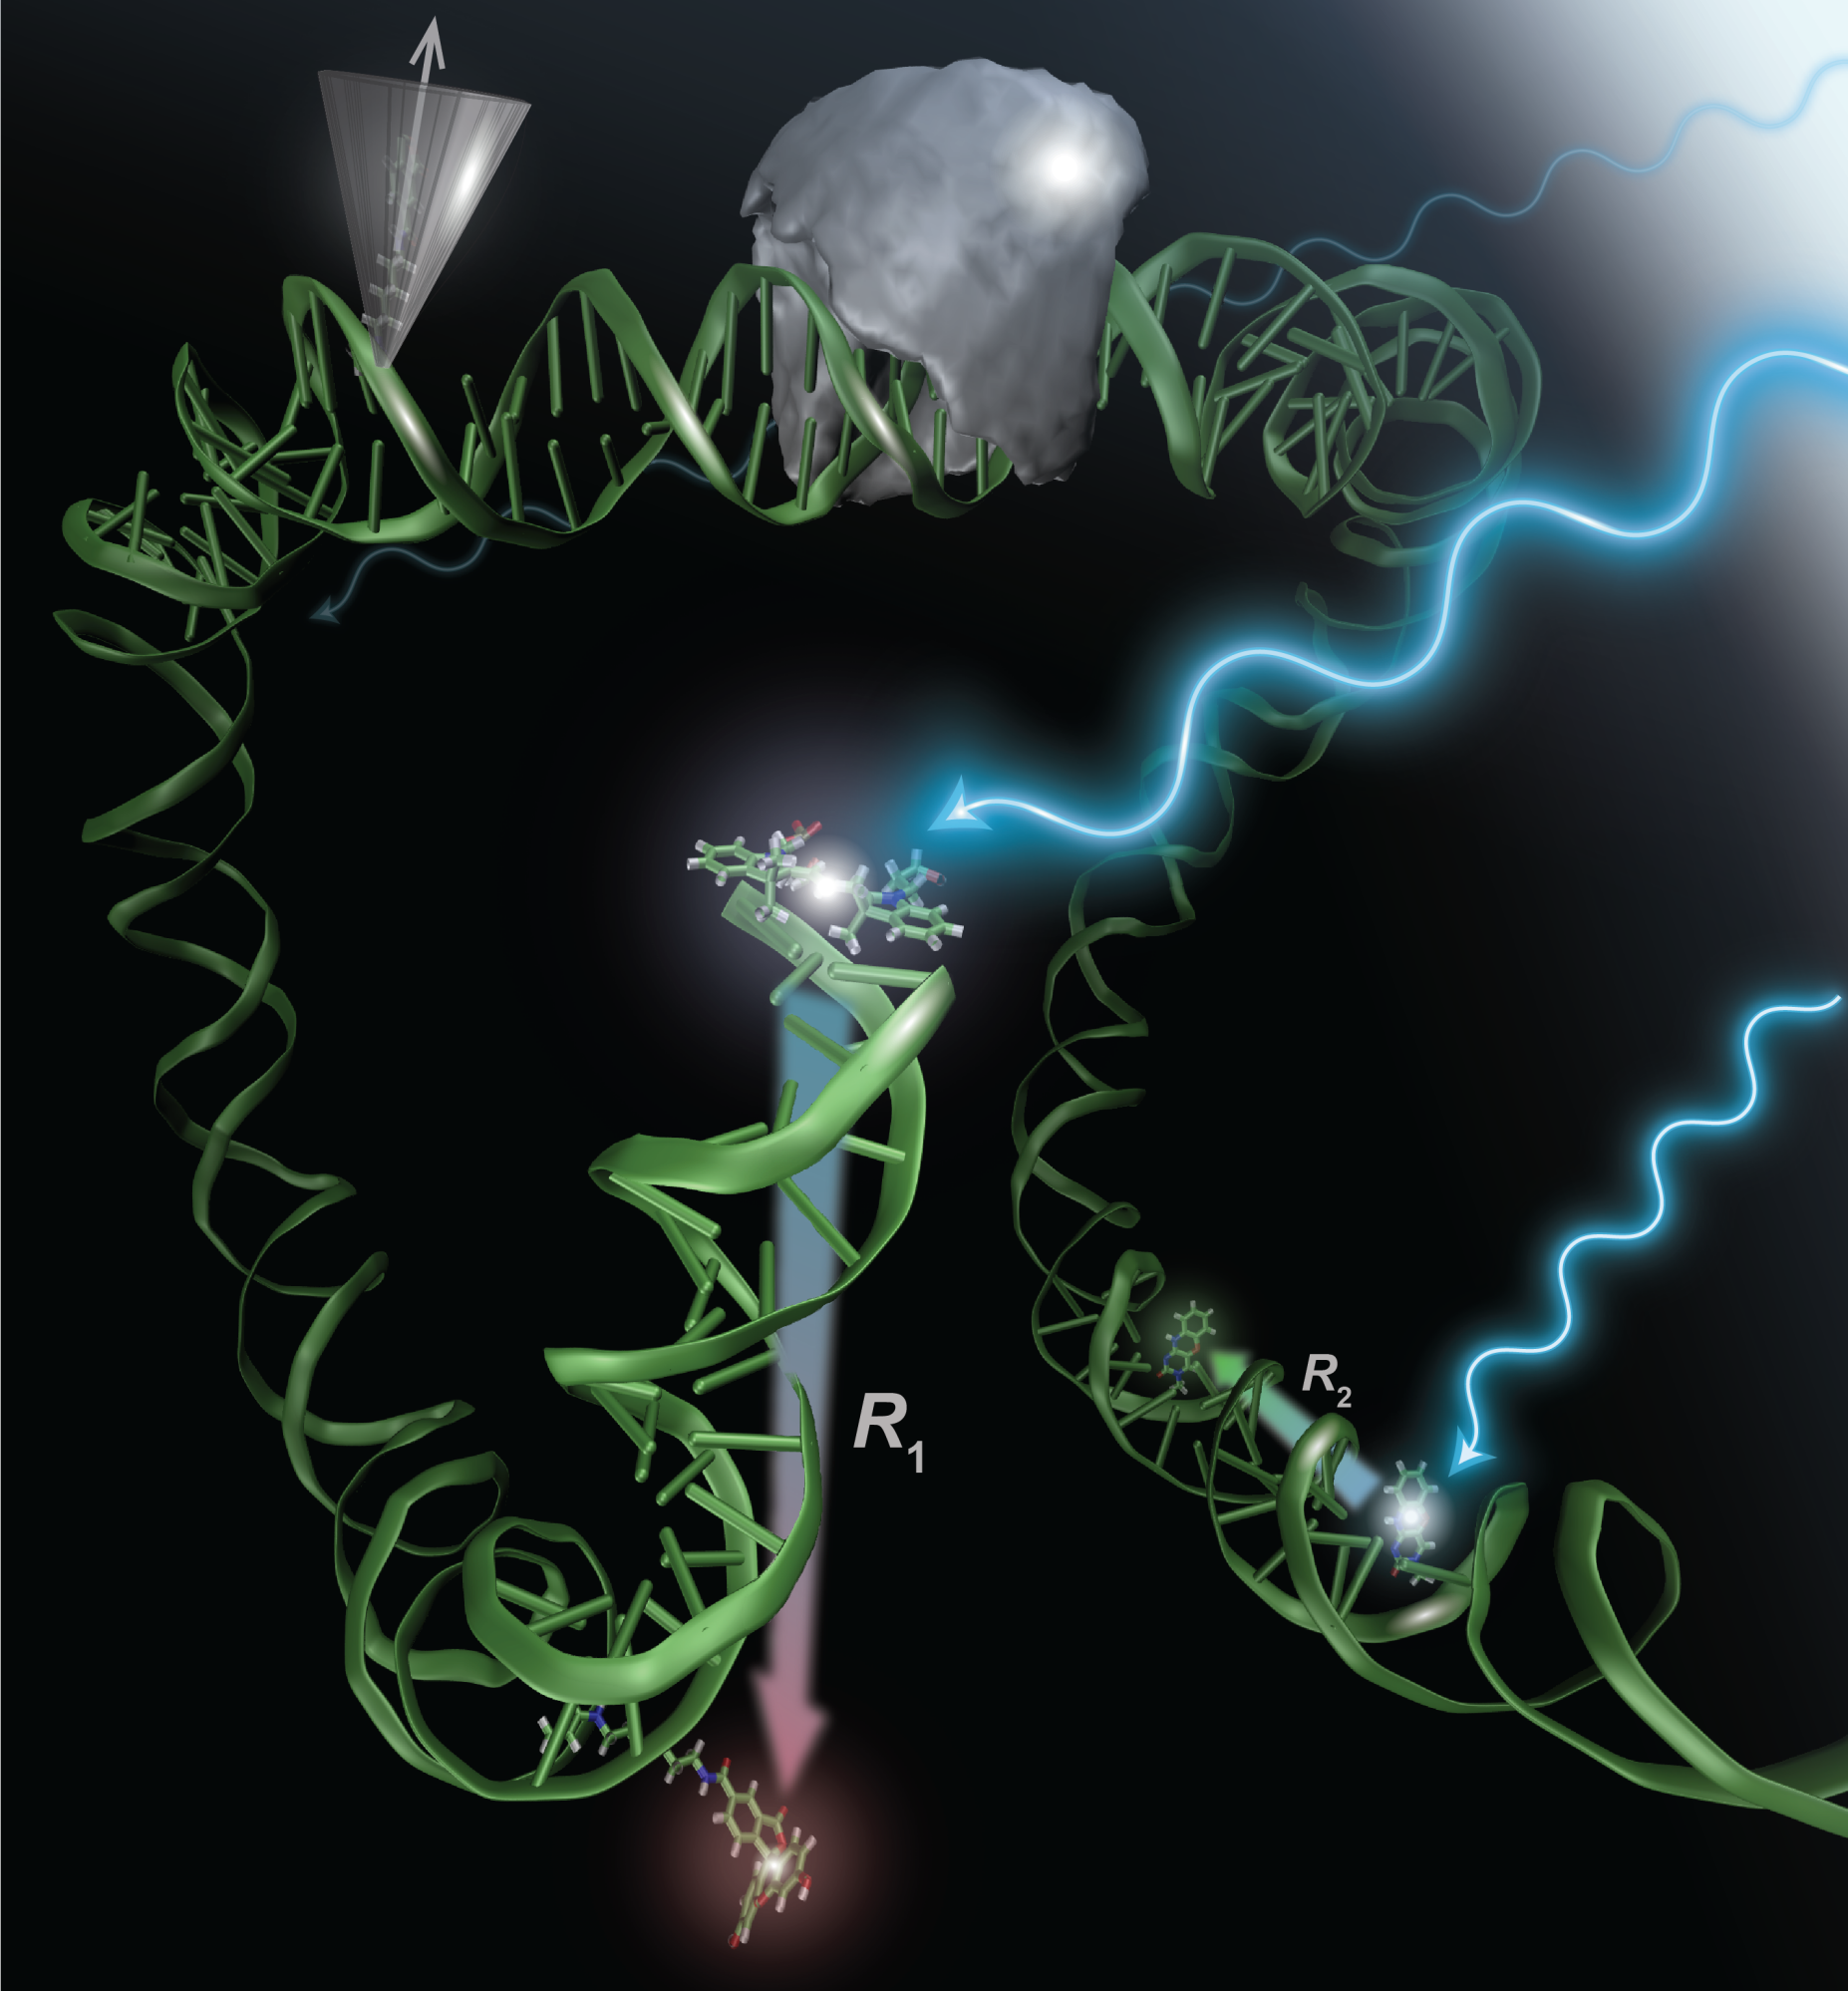
\includegraphics[width=0.7\textwidth]{adds//cbc_fig2.png}
    \captionsetup{width=.95\textwidth}
    \caption{Frontispiece for Paper I.}
    \label{Fig:chap_Papers_CBC}
\end{figure}

 \paragraph{Preparation of figures.} Information or courses on how scientific illustrations are prepared are rarely available. Students are thus often oblivious when preparing such visuals (including myself), which is unfortunate since illustrative figures greatly reduces the time required to understand the paper. This short section addresses the issue in the context of the frontispiece of Paper I (Figure \ref{Fig:chap_Papers_CBC}). A detailed step-by-step tutorial including all the raw data files and sessions is found at

 \url{www.fluortools.com/misc/scientific-illustration}

 In summary, a DNA coordinate file was first constructed by w3DNA\cite{Zheng2009} using a manually edited input file describing all base-pair step parameters in the structure. Using Avogadro\cite{Hanwell2012}, the DNA molecule file was then combined with an accessible volume (AV) coordinate file of Alexa488 attached to DNA. Individual dye coordinates were constructed using ChemBio3D\cite{ChemBio3D} and positioned at the desired sites in the molecule file using Avogadro. The DNA molecule file, including the AV and dyes, was then visualized in VMD\cite{VMD} producing a POV-Ray file for high resolution rendering in POV-Ray\cite{POVray}. The rendered png file was then edited using Adobe Illustrator in order to add light waves, dye-glow, the transition moment-cone and FRET arrows. To get the feeling that the arrows lie within the molecule, several figure frames with and without arrows were combined using Paint Shop Pro.

% \paragraph{DNA molecule figures.} The DNA molecule files were constructed using a combination of w3DNA, ChemBio3D and Avogadro. The molecules were rendered using VMD and POV-Ray. Arrows denoting FRET were added to the rendered figures using Illustrator and finally post-edited using Paint Shop Pro. The depiction of different transition moment reorientation models in Figure 7a-c where made in Illustrator. The molecule files in Figure 7d-e were kindly supplied by Prof. Claus Seidel's group and rendered in VMD.
%
% \paragraph{Online mini-TOC figure.} This figure is shown in Figure \ref{Fig:chap_Papers_CBC}. The DNA molecule was synthesized using HyperChem, rendered in VMD and post-edited in Illustrator. The greyscale floppy ends were made by overlaying two DNA figures.
%
\section{Paper II}
 Paper II describes the characterization of nucleobase analogue tC$_\mathrm{nitro}$ with particular focus put on its use as a FRET acceptor with tC or tC$^\mathrm{O}$ serving as the donor. The paper builds upon the findings of the 2009 JACS paper provided in Appendix 1 by further elucidating the properties of tC$_\mathrm{nitro}$ under biological conditions.

 \paragraph{Motivation and most important findings.} In order to simulate and interpret base-base FRET experiments quantitatively, the number of electronic transitions within the lowest energy absorption band of tC$_\mathrm{nitro}$ had to be determined as well as the orientation of the transition dipole moment vectors within the molecular framework. In other words, the number of antennas involved in FRET and their directions had to be known. Paper II reports in particular these two findings (shown in Figure \ref{Fig:chap_Papers_JPCB}). Using a combination of TDDFT calculations, MCD and the fundamental fluorescence anisotropy recorded in low temperature glass, the lowest energy absorption band of tC$_\mathrm{nitro}$ was shown to be the result of a single electronic transition. From the LD of tC$_\mathrm{nitro}$ aligned in stretched PVA film combined with TDDFT calculations, the direction of the lowest energy transition dipole moment of tC$_\mathrm{nitro}$ was found to be oriented 27$^\circ$ towards the NO$_2$-group from the molecular long axis. The paper additionally shows that the pK$_\mathrm{a}$ of tC$_\mathrm{nitro}$ is 11.1 (deprotonation at the central enamine involved in Watson-Crick H-bonding) which led us to the conclusion that the neutral, Watson-Crick active form is totally predominant at biological conditions. While tC$_\mathrm{nitro}$ is virtually non-fluorescent in aqueous solution at room temperature, the absorption spectrum of tC$_\mathrm{nitro}$ neatly overlaps the emission spectra of both tC and tC$^\mathrm{O}$ (Figure \ref{Fig:chap_Papers_JPCB2}). The spectral overlap integrals in DNA were found to be $J=5.4\times 10^{13}$ and $J=1.2\times10^{14}$ resulting in critical Förster distances of $R_0=23.4$ Å and $R_0=27.2$ Å, respectively, with the assumption of $\kappa^2 = \frac{2}{3}$.
\begin{figure}
    \centering
        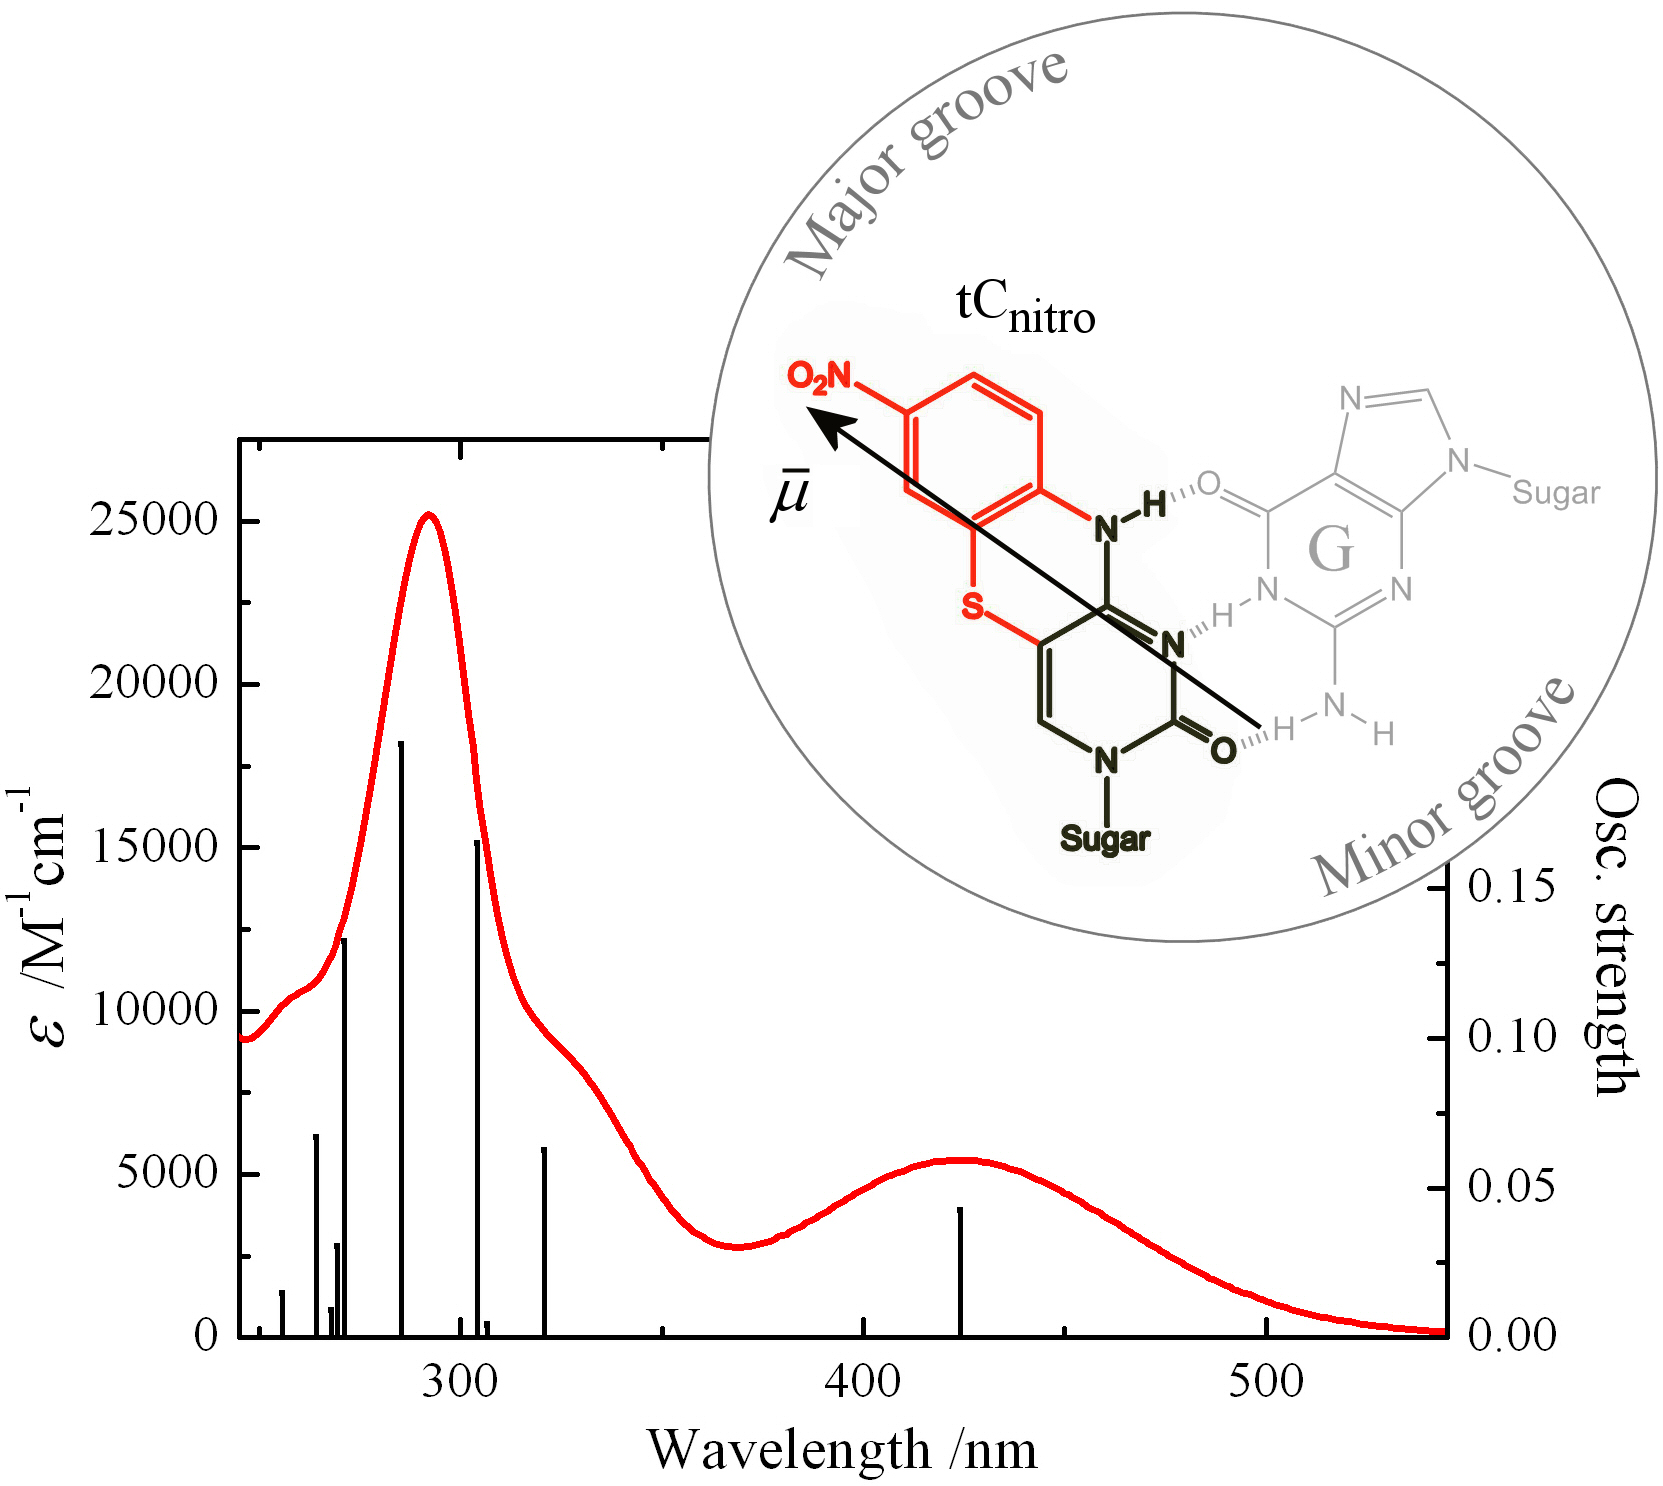
\includegraphics[width=0.65\textwidth]{adds//jpcb_fig.jpg}
    \captionsetup{width=.95\textwidth}
    \caption{The absorption spectrum of tC$_\mathrm{nitro}$ in H$_2$O along with the TDDFT predicted electronic transitions. The most important finding of Paper II is the direction of the lowest energy transition dipole moment of tC$_\mathrm{nitro}$ (insert)}
    \label{Fig:chap_Papers_JPCB}
\end{figure}
\begin{figure}
    \centering
        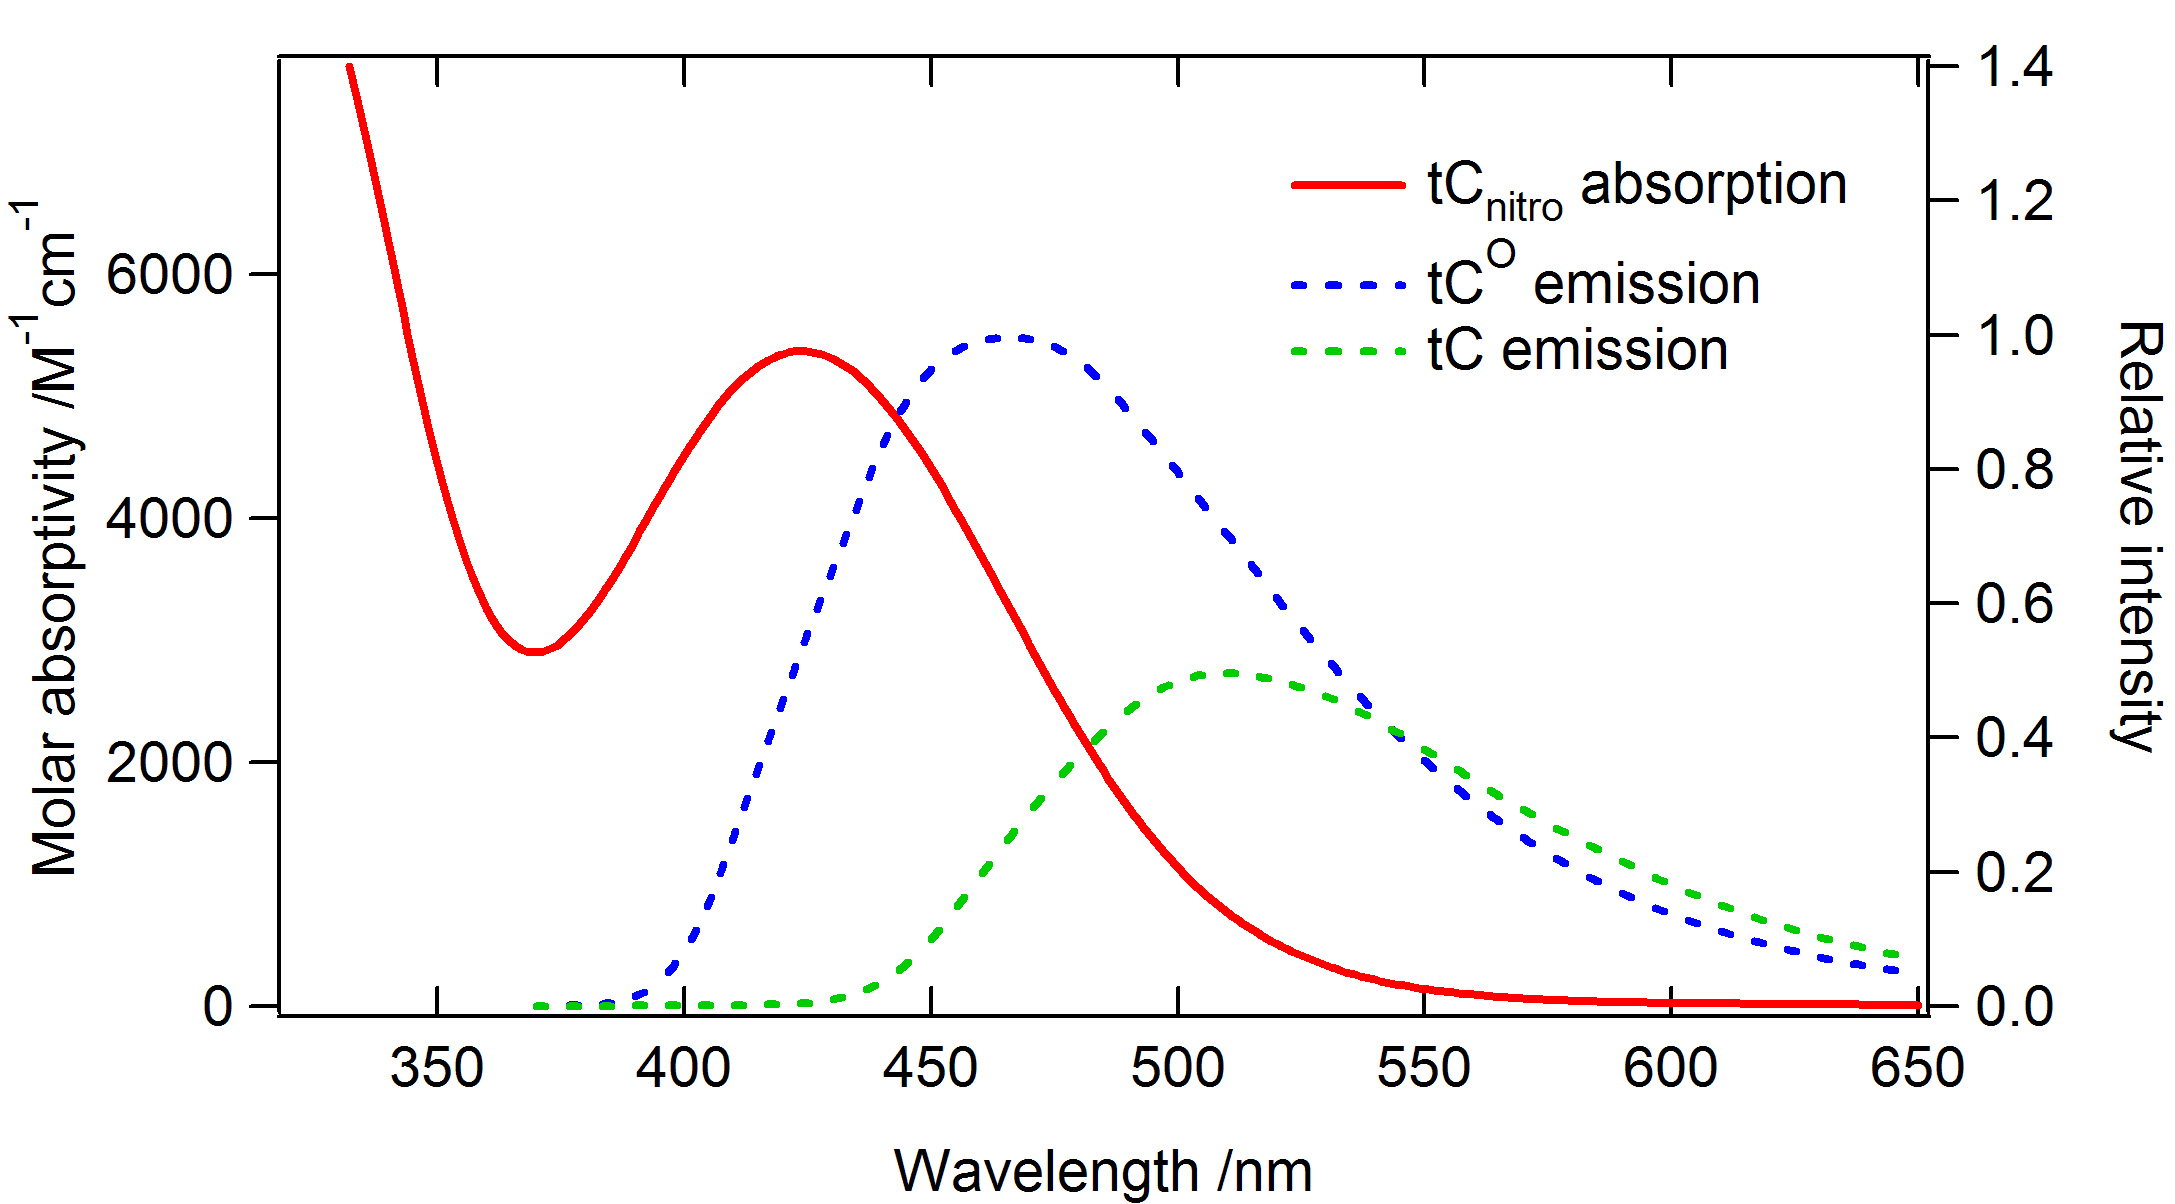
\includegraphics[width=0.8\textwidth]{adds//jpcb_fig2.png}
    \captionsetup{width=.95\textwidth}
    \caption{Spectral overlap between the absorption spectrum of tC$_\mathrm{nitro}$ and the emission spectra of tC and tC$^\mathrm{O}$.}
    \label{Fig:chap_Papers_JPCB2}
\end{figure}

\section{Paper III}
 Paper III describes a new computational method for the simulation and analysis of FRET in nucleic acids. The method is generic in the sense that it can be used to simulate and analyse FRET quantitatively between any two probes positioned in any nucleic acid geometry. However, the method is particularly powerful for modelling constrained probes such as base-base FRET.

 \paragraph{Motivation.} In the first paper reporting base-base FRET (Appendix 1), the data was analysed by expressing the FRET efficiencies between multiple donor-acceptor pairs in dsDNA as a function of donor-acceptor separation.\cite{Borjesson2009a} This modelling was possible due to the simple sequential 5'-3' increase in donor-acceptor separation combined with the well-known helical periodicity of regular B-DNA. This model system results in a sinusoidal oscillation of the FRET efficiency as the number of bases in between the FRET-pair increases and, indeed, the experimental results showed that the structure in which the probes were positioned corresponded to a regular B-DNA helix (Figure \ref{Fig:chap_intro_basefretgraph}). However, in an actual FRET experiment the structure is rarely a simple periodic helix but rather completely or partly unknown. This makes it inherently complicated to model FRET between probes in constrained environments where the assumption of freely rotating fluorophores (i.e. $\kappa^2=\frac{2}{3}$) is no longer valid. In other words, there are always two unknown parameters for each measured FRET efficiency: $R$ and $\kappa^2$ (in the method used in Appendix 1 there were essentially only one parameter since $R$ was known in advance). Without a fundamentally new methodology capable of simulating both probe orientation and position in any nucleic acid structure, it would be impossible to interpret actual base-base FRET experiments quantitatively.

 \paragraph{The principle of the method.} FRETmatrix is build on a rigorous, matrix-based nucleic acid structure scheme called the Cambridge University Engineering Department Helix Computation Scheme (CEHS). In short, a 3D nucleic acid geometrical model is build by defining six rigid-body parameters describing each base-pair in the structure: three rotations (buckle, propeller, opening) and three translations (shear, stretch, stagger), as well as six rigid-body parameters describing each dinucleotide step in the structure: three rotations (tilt, roll, twist) and three translations (shift, slide, rise). By replacing one of the canonical bases in the modelled structure with a base probe, the position and orientation of the transition dipole moment of the dye can be accurately described at any site within the nucleic acid. Then, knowing the 3D coordinates describing the position and orientation of all transition dipole moments within the modelled nucleic acid structure, the energy transfer rate constants are simulated using the well-known Förster equations.

 In order to interpret base-base FRET experiments quantitatively the rotational dynamics of the base probes must be known or included in the analysis. Such fast dynamics is an inherent property of the nucleobases and not a unique property of the dyes. In FRETmatrix, rotational dynamics is modelled by assigning two different energy potentials to the in-plane and out-of-plane movement of the bases in their base-pairing environment within dsDNA (Figure \ref{Fig:chap_Papers_NAR}). The distribution of transition dipole moments in a given ensemble experiment is then described by the Boltzmann distribution along each of the two coordinates. The result is a directional vector distribution representing the orientation of a probe during an energy transfer event (Figure \ref{Fig:chap_Papers_NAR}).

\begin{figure}
    \centering
        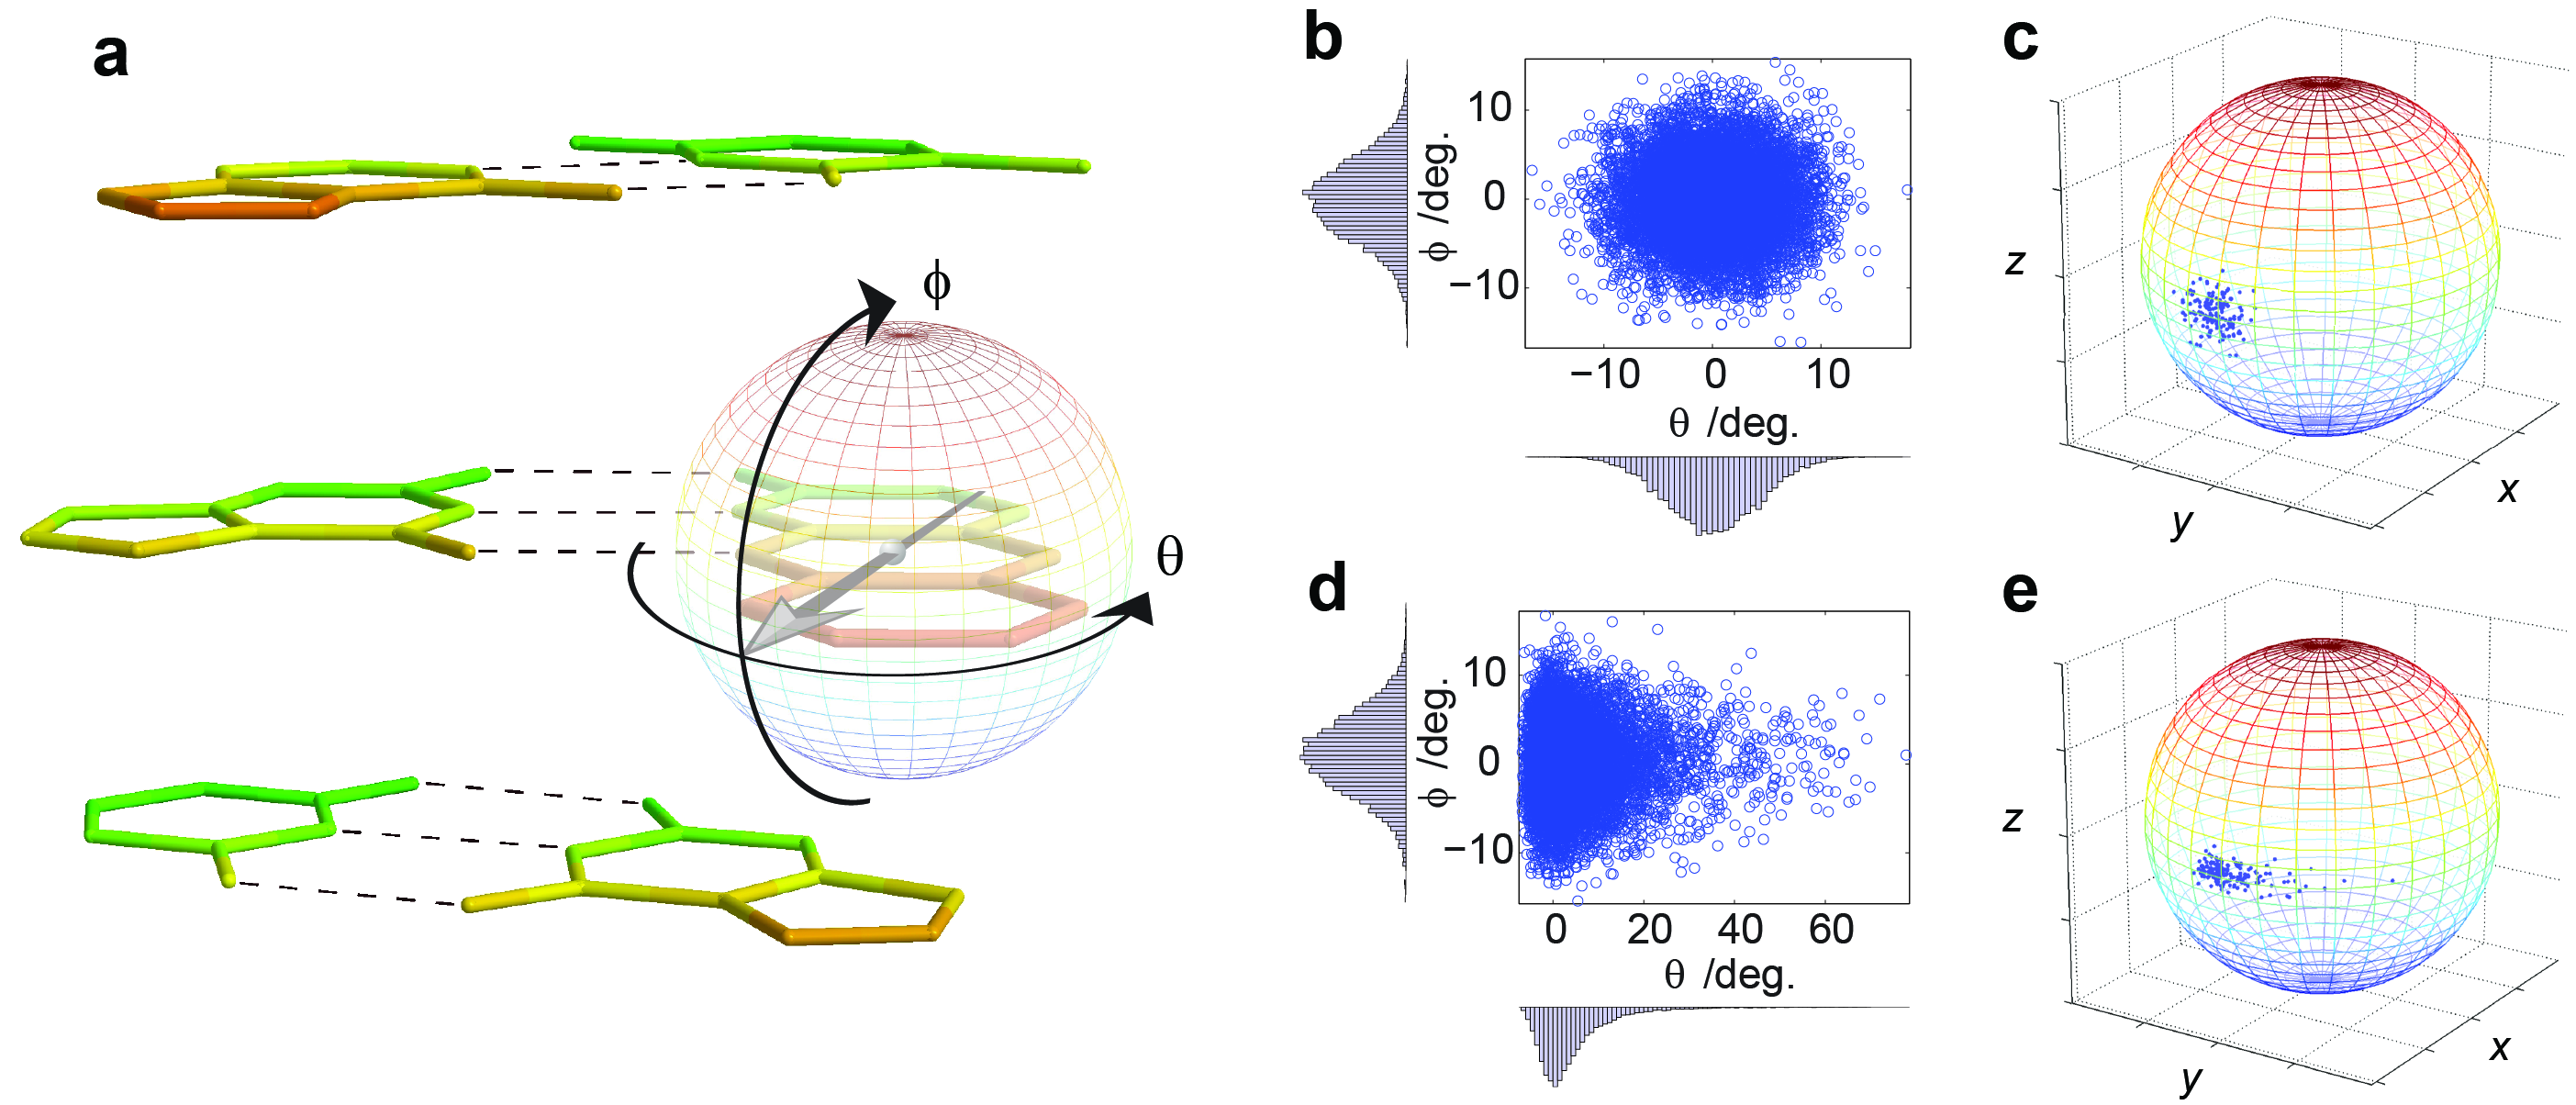
\includegraphics[width=0.95\textwidth]{adds//nar_fig.png}
    \captionsetup{width=.95\textwidth}
    \caption{Representing local dye rotational dynamics by directional vector distributions. a) Definition of in-plane and out-of-plane movement of the base. b-c) Representing $\theta$ and $\phi$ by Gaussian distributions. d-e) Representing the out-of-plane coordinate by a Gaussian distribution and in-plane coordinate by the Boltzmann distribution for a harmonic potential.}
    \label{Fig:chap_Papers_NAR}
\end{figure}

 \paragraph{Experimental demonstration studies.} Since any set of structural or dynamical parameters can be defined as the unknowns in a given experiment, the method is highly flexible. In demonstration study 1 of Paper III donor-acceptor pairs were positioned in regular dsDNA in which case the overall nucleic acid geometry was known in advance. This allowed us to analyze the experimental data, being all the donor intensity decays, in terms of the local probe dynamics. The results revealed directional vector distributions in excellent agreement with those expected for bases positioned within dsDNA. In addition, the results showed that the probes were bent towards the 3' end and into the major groove as predicted by TDDFT calculations in Paper V.

 In demonstration study 2 of Paper III we used the information gained in demonstration study 1 and probed the 3D geometry of two local sites in DNA. Here, the model structures were deliberately chosen to be as simple as possible representing more complex geometries such as a protein binding site, a DNA lesion, a mismatch site, an RNA junction or some other local structural perturbation.

 \paragraph{The software.} To many people seeking to use base-base FRET for their own studies, the FRETmatrix methodology was in large parts too laborious to implement. Large amounts of effort was therefore put into making the method available to other researchers but ourselves and the result was a MATLAB-based software equipped with a user-interface and a user-guide (Supplementary Note 3 in Paper III). The software is described further in section \ref{sec_PublishedSoftware}. A one page brief summary of the software was made for the 2012 Autumn newsletter of Glen Research (Appendix 2).

\section{Paper IV}
 In Paper IV we report a simple DNA based adjustable strap capable of existing in five different states, each state accessed reversibly and with distinct fluorescence readouts.

 \paragraph{Motivation.} The ability to program readable information into nanoscale devices is an attractive technological advance in several aspects. Firstly, as a long-term information storage medium, DNA is stable and extremely dense (think of the amount of information coded into the human genome!). Methods capable of rapidly programming and reading information from such media are thus highly attractive.\cite{Church2012,Wong2003,Portney2008} Secondly, functional molecular machines capable of responding to an external stimuli are attractive as sensors,\cite{Zhang2007b} long-range transport\cite{Wickham2012,Wickham2011,Lund2010,Douglas2012,Andersen2009} and even computing\cite{Zhang2007a,Stojanovic2002,Qian2011}.

 \paragraph{Principles of the switch.} The switch consists of a 45 bp long single DNA strand divided into four repeating TAAT-ATTA box sequences plus an additional 13 base long tail. A FRET donor and acceptor is attached at either end of the TAAT-ATTA region which serves to signal the state of the switch. The repeating TAAT-ATTA region is self-complementary and thus has four different local equilibrium hairpin (stem-loop) structures characterized by different stem lengths (Figure \ref{Fig:chap_Papers_CC}a). The four different hairpin structures constitute four of the five states. The fifth state is the fully opened hairpin obtained by the addition of the 45 bp long fully complementary strand. The state of the switch is the state with the lowest overall free energy of the system, which is controlled by adding the appropriate complementary strands of different lengths to the switch (blue strands in Figure \ref{Fig:chap_Papers_CC}a). If no complementary strands are added the main strand (red strand in Figure \ref{Fig:chap_Papers_CC}a) is folded into the longest possible hairpin structure, i.e. state 5. This DNA-based strategy for creating a dynamic switch is called strand-displacement and has been exploited in numerous previous reconfigurable nanostructures.\cite{Zhang2011}

\begin{figure}
    \centering
        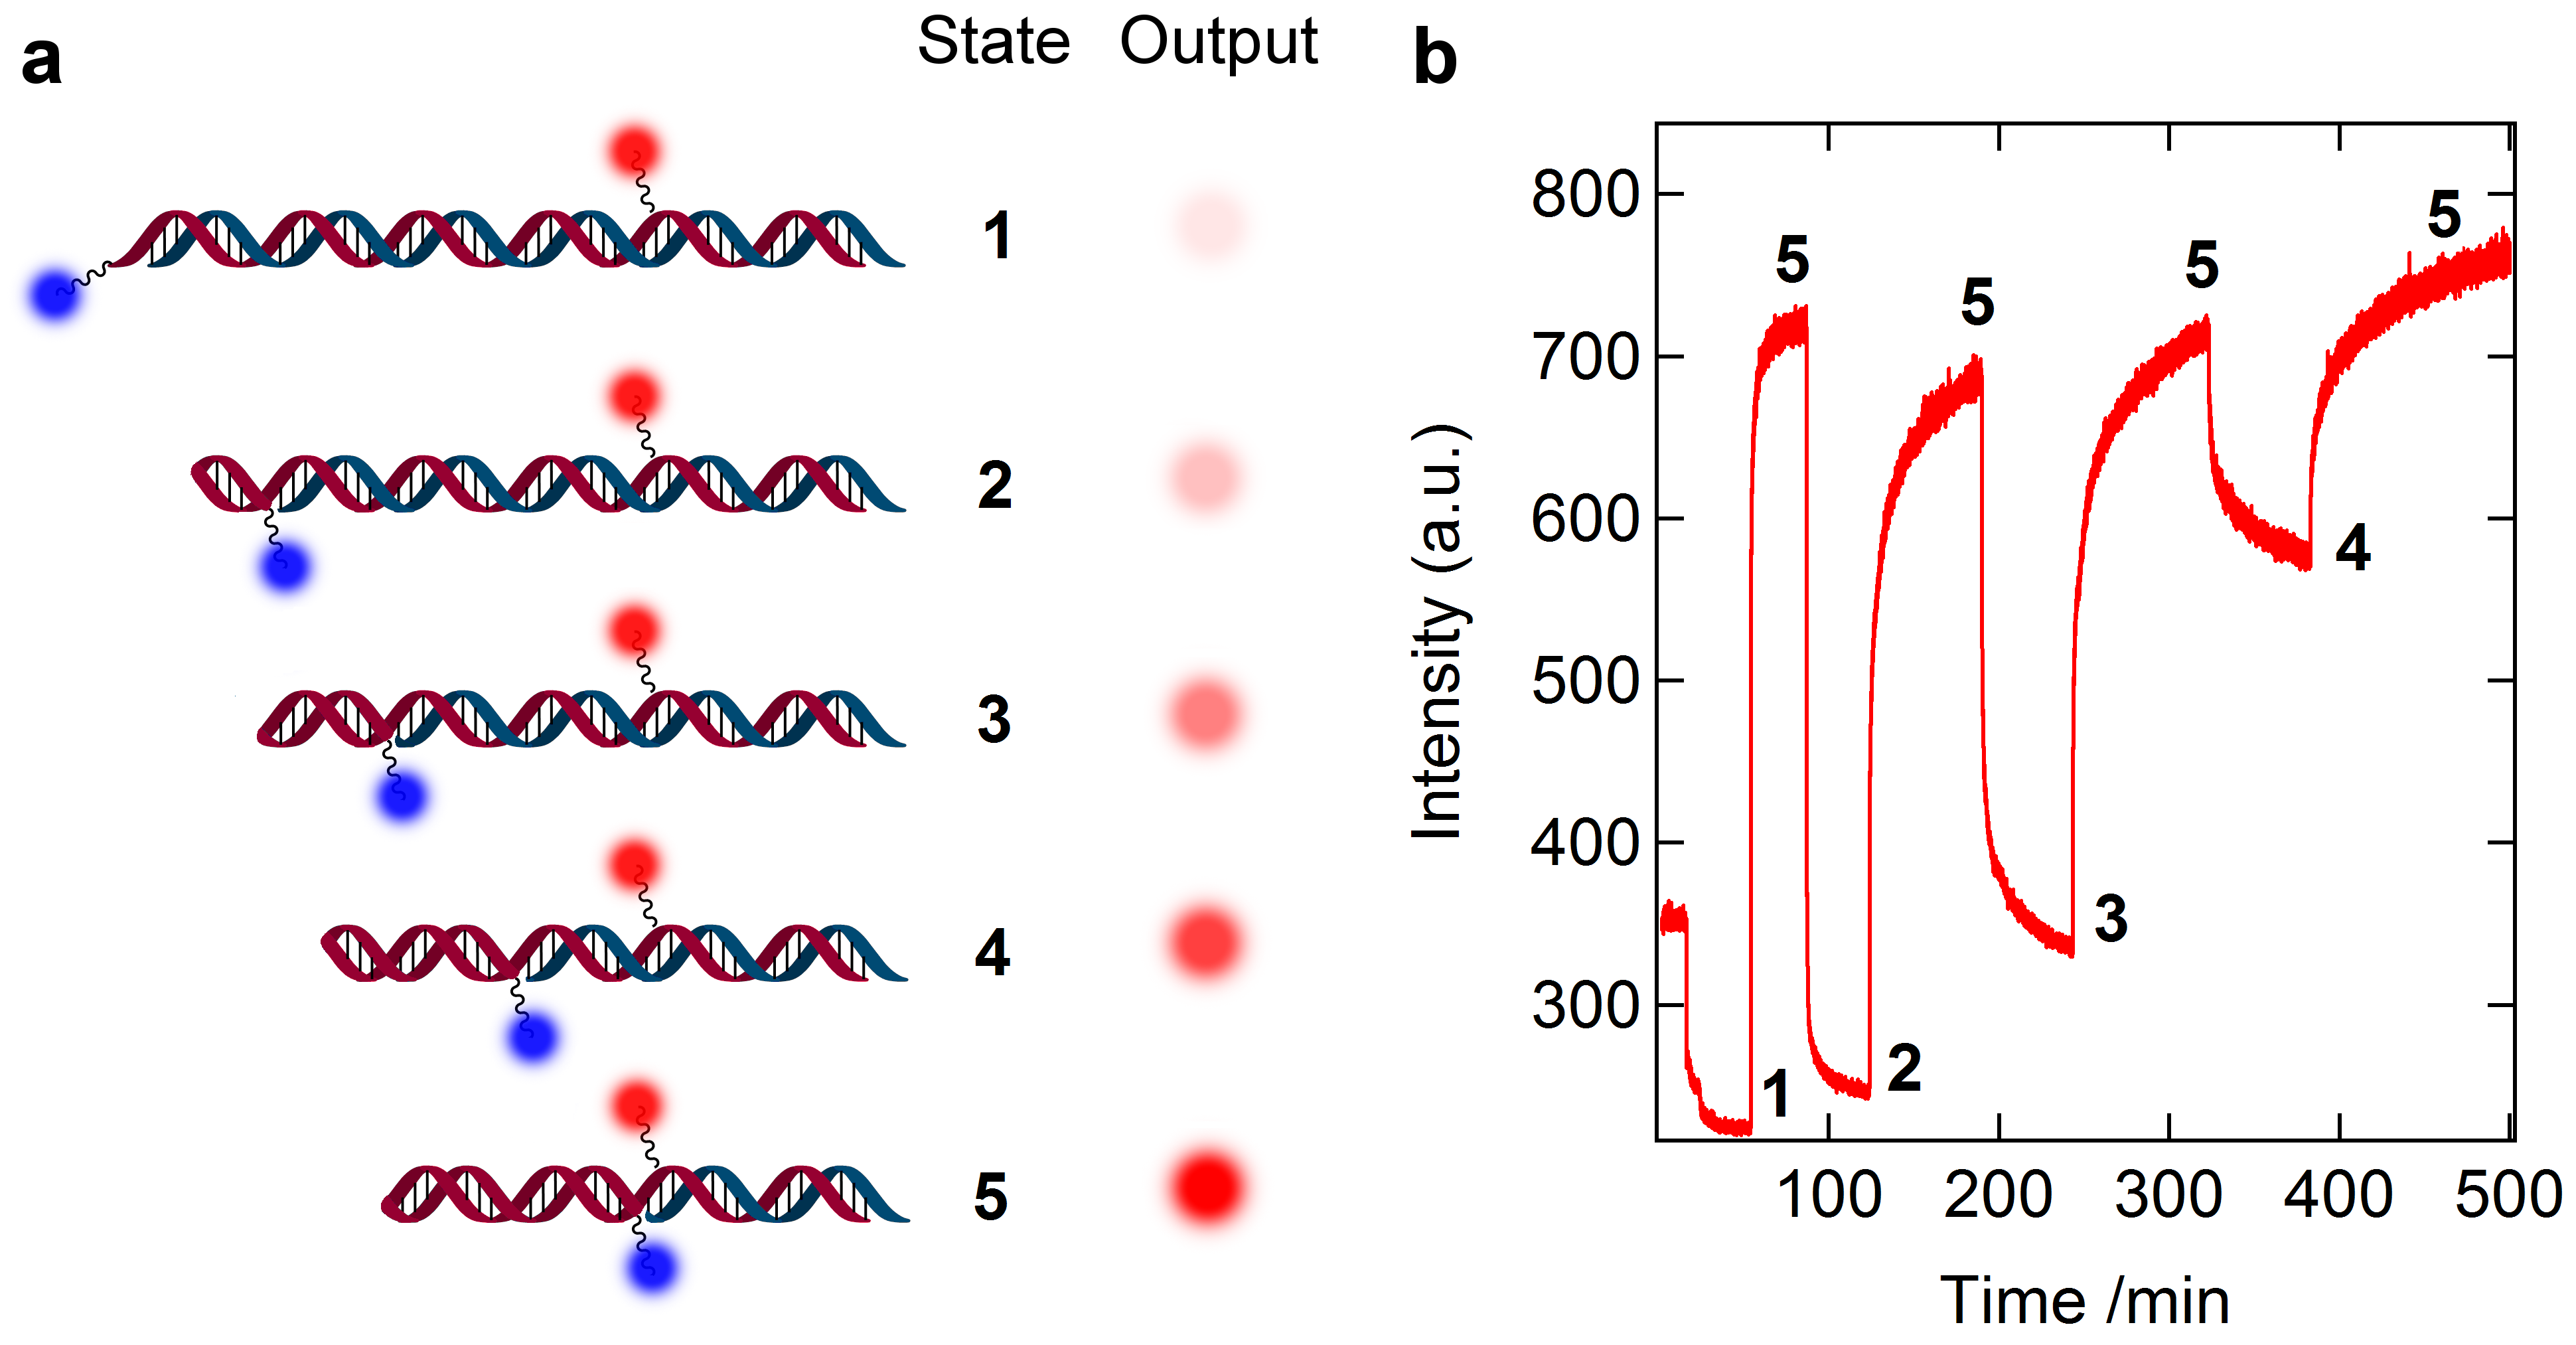
\includegraphics[width=1\textwidth]{adds//cc_fig.png}
    \captionsetup{width=.95\textwidth}
    \caption{The DNA switch of Paper IV. a. The five different states giving rise to a change in the fluorescence output. The red strand is the main strand functionalized with a FRET donor (blue) and a FRET acceptor (red) at either end of a TAAT-ATTA repeat region. The blue strands are complementary strands of different lengths. The output signal is the acceptor intensity upon donor excitation. b. Demonstration of accessing the five different states of switch (from Figure 3 in Paper IV). The graph shows the intensity from the acceptor upon donor excitation. The reversibility is obtained by elongating the blue complementary strands with an overhang which is the target of a third strand (release-strand) added at each of the lower plateaus.}
    \label{Fig:chap_Papers_CC}
\end{figure}

 \paragraph{Demonstration studies.} All experiments were performed by J. Burns and E. Stulz. The demonstration studies show that the state of the switch can be set and altered at will by the addition of the proper navigation strands to the solution containing the switch. The combination of theoretical FRET calculations performed using FRETmatrix combined with FRET efficiencies measured for the different states of the switch proves that the switch exists in the expected pre-defined states. The reversibility of the switch is demonstrated by monitoring the relative fluorescence intensity from the acceptor upon donor excitation as the complementary strands are added sequentially to the solution (Figure \ref{Fig:chap_Papers_CC}b). When the signal is high the donor and acceptor is brought close together, which corresponds to a long stem hairpin, while the signal is low when the donor and acceptor is located far from one another, which corresponds to a short stem hairpin.

\section{Paper V}
 Paper V reports new insight into the electronic and structural properties of the tC bases (tC, tC$^\mathrm{O}$ and tC$_\mathrm{nitro}$).

 \paragraph{Motivation.} This work was motivated by two driving forces. Firstly, the high, relatively stable fluorescence properties and single-exponential fluorescence decays of the tC and tC$^\mathrm{O}$ bases in DNA are unique features of these dyes compared to almost all other dyes positioned in DNA. It is thus not just of fundamental interest but also highly useful when designing new and improved fluorescent DNA modification to understand why tC and tC$^\mathrm{O}$ exhibit such desirable properties while tC$_\mathrm{nitro}$ is virtually non-fluorescent at room temperature in aqueous solution. Secondly, in order to understand the behaviour of the tC probes in various confined biological environments, as well as to interpret FRET and fluorescence anisotropy experiments involving these probes, the molecular geometries and structural dynamics of the probes had to be known.

 \paragraph{Insight into the excited state decay pathways.} The excited state relaxation processes of the tC probes were investigated by a combination of temperature-dependent fluorescence quantum yield measurements, TDDFT calculations and solvatochromic experiments.
%We found that while tC$_\mathrm{nitro}$ is non-fluorescent at room temperature tC$_\mathrm{nitro}$ starts to fluoresce at lower temperatures with a maximum fluorescence quantum yield plateau of $\Phi_\mathrm{f} = 0.21$ (Figure 2 in Paper V).
 Using an Arrhenius expression to describe the temperature-dependent non-radiative decay process of tC$_\mathrm{nitro}$, we found that the reason tC$_\mathrm{nitro}$ is non-fluorescent at room temperature is due to an efficient IC from the first excited state, very likely being directly associated with twisting of the NO$_2$ group. This decay pathway was characterized by means of TDDFT calculations which provided insight into the electronic structure and potential energy surfaces along the NO$_2$ rotational coordinate of tC$_\mathrm{nitro}$ (Figure 8 in Paper V). The results showed that the excited state dipole moment of tC$_\mathrm{nitro}$ increases as the NO$_\mathrm{2}$ group rotates leading to a higher activation energy for this process in non-dipolar solvents. In other words, as the dipolarity of the solvent increases the activation barrier for IC decreases leading to a lower fluorescence quantum yield of tC$_\mathrm{nitro}$. The result is that tC$_\mathrm{nitro}$ is non-fluorescent in dipolar solvents such as H$_2$O and fluorescent in less dipolar solvents such as THF and dioxane (Figure 9 in Paper V).

 The temperature-dependent experiments were performed using a temperature-controlled Oxford Cryostat mounted in a fluorescence spectrophotometer. At this point the reader is warned: Doing quantitative spectroscopy at low temperatures can be time consuming and non-trivial. At low temperatures the sample often precipitates and the cuvette may break as a result of tensions in the formed glass. In such cases the cryostat can get severely contaminated if not properly evacuated. In addition, it is a tedious task to obtain perfect baselines of the cryostat at all temperatures.

\begin{figure}
    \centering
        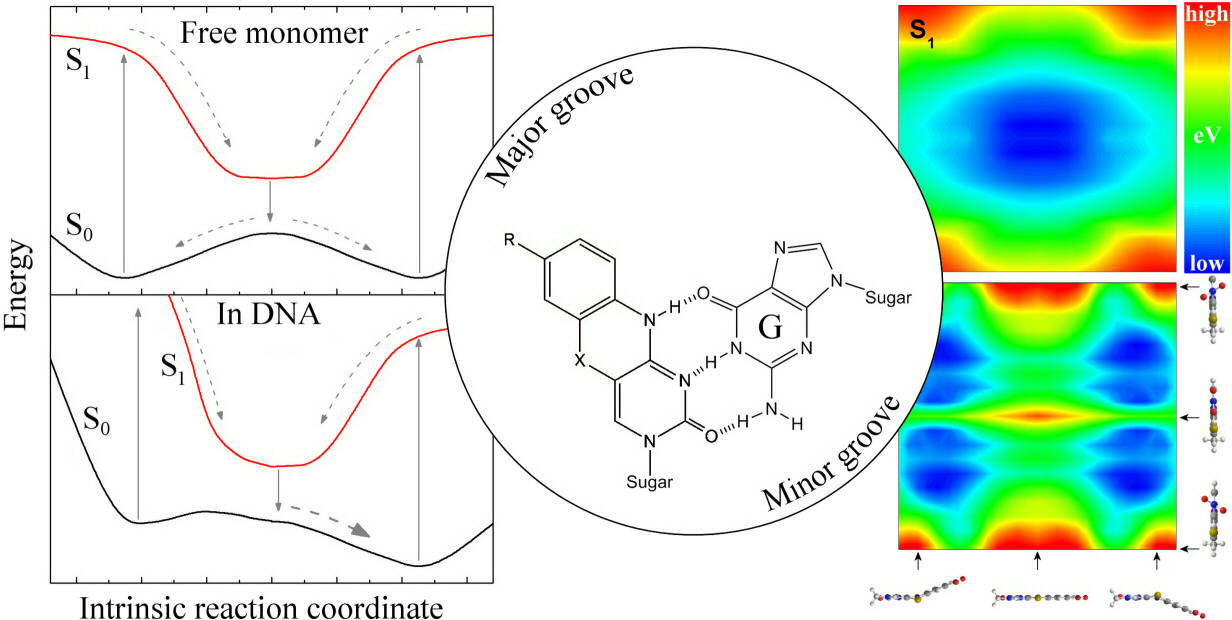
\includegraphics[width=0.8\textwidth]{adds//pccp_fig.jpg}
    \captionsetup{width=.95\textwidth}
    \caption{The most important finding of Paper V is the potential energy surfaces of tC, tC$^\mathrm{O}$ and tC$_\mathrm{nitro}$. Left: Proposed potential energy surfaces of tC$_\mathrm{nitro}$ in its free monomeric form (predicted by TDDFT) and after insertion into double-stranded, B-form DNA (proposed model). Rigth: Potential energy surfaces of tC$_\mathrm{nitro}$ following the coordinate corresponding to folding along the middle S-N axis and the coordinate corresponding to twisting of the NO$_2$-group.}
    \label{Fig:chap_Papers_PCCP}
\end{figure}

 \paragraph{Insight into the molecular structures.} Insight into the potential energy surfaces of all three probes were obtained by means of TDDFT calculations (Figure \ref{Fig:chap_Papers_PCCP}). It was found that all three bases possess a low energy intrinsic reaction coordinate corresponding to folding along the central S-N axis of tC and tC$_\mathrm{nitro}$ and O-N axis of tC$^\mathrm{O}$ (Figures 5-7 in Paper V). In short this means that the tC bases are highly flexible in terms of bending along this central axis. While this result at first glance may seem uninteresting, this low energy IRC of the tC bases very likely dictates the geometrical appearance of the bases in constrained biological environments and thus their ability to adapt sterically into various biological systems such as DNA-protein complexes (Figure 10 in Paper V). In addition the bending property of the tC probes has a profound effect in the interpretation of FRET experiments, and this model was confirmed experimentally in Paper III.

\section{Paper VI}
 Paper VI reports the development of a new fluorescent adenine analogue, qA, and describes it photophysical and base-mimicking properties in DNA.

 \paragraph{Motivation.} Since we had fluorescent cytosine base analogues only, namely tC and tC$^\mathrm{O}$, we were highly interested in expanding the fluorescent nucleobase arsenal with dyes mimicking the base-pairing of adenine, guanine, or thymine. Such additions would facilitate a more versatile fluorescence toolbox and simplify systems design in e.g. FRET experiments.

 \paragraph{Design of fluorescent DNA base analogues.} Prior synthesizing qA, a theoretical nucleobase analogue library was constructed which served as a source of inspiration in the development of new, potentially fluorescent, DNA base analogues (Appendix 3). Due to synthetic difficulties, qA was the only structure from the library which resulted in a phosphoramidite for oligonucleotide synthesis. Several other molecular structures from the library, however, are equally or even more interesting as seen from a fluorescence application point of view. The qA structure was also derived by Marcus independently of the base library at the same time qA was added to the library.

\begin{figure}
    \centering
        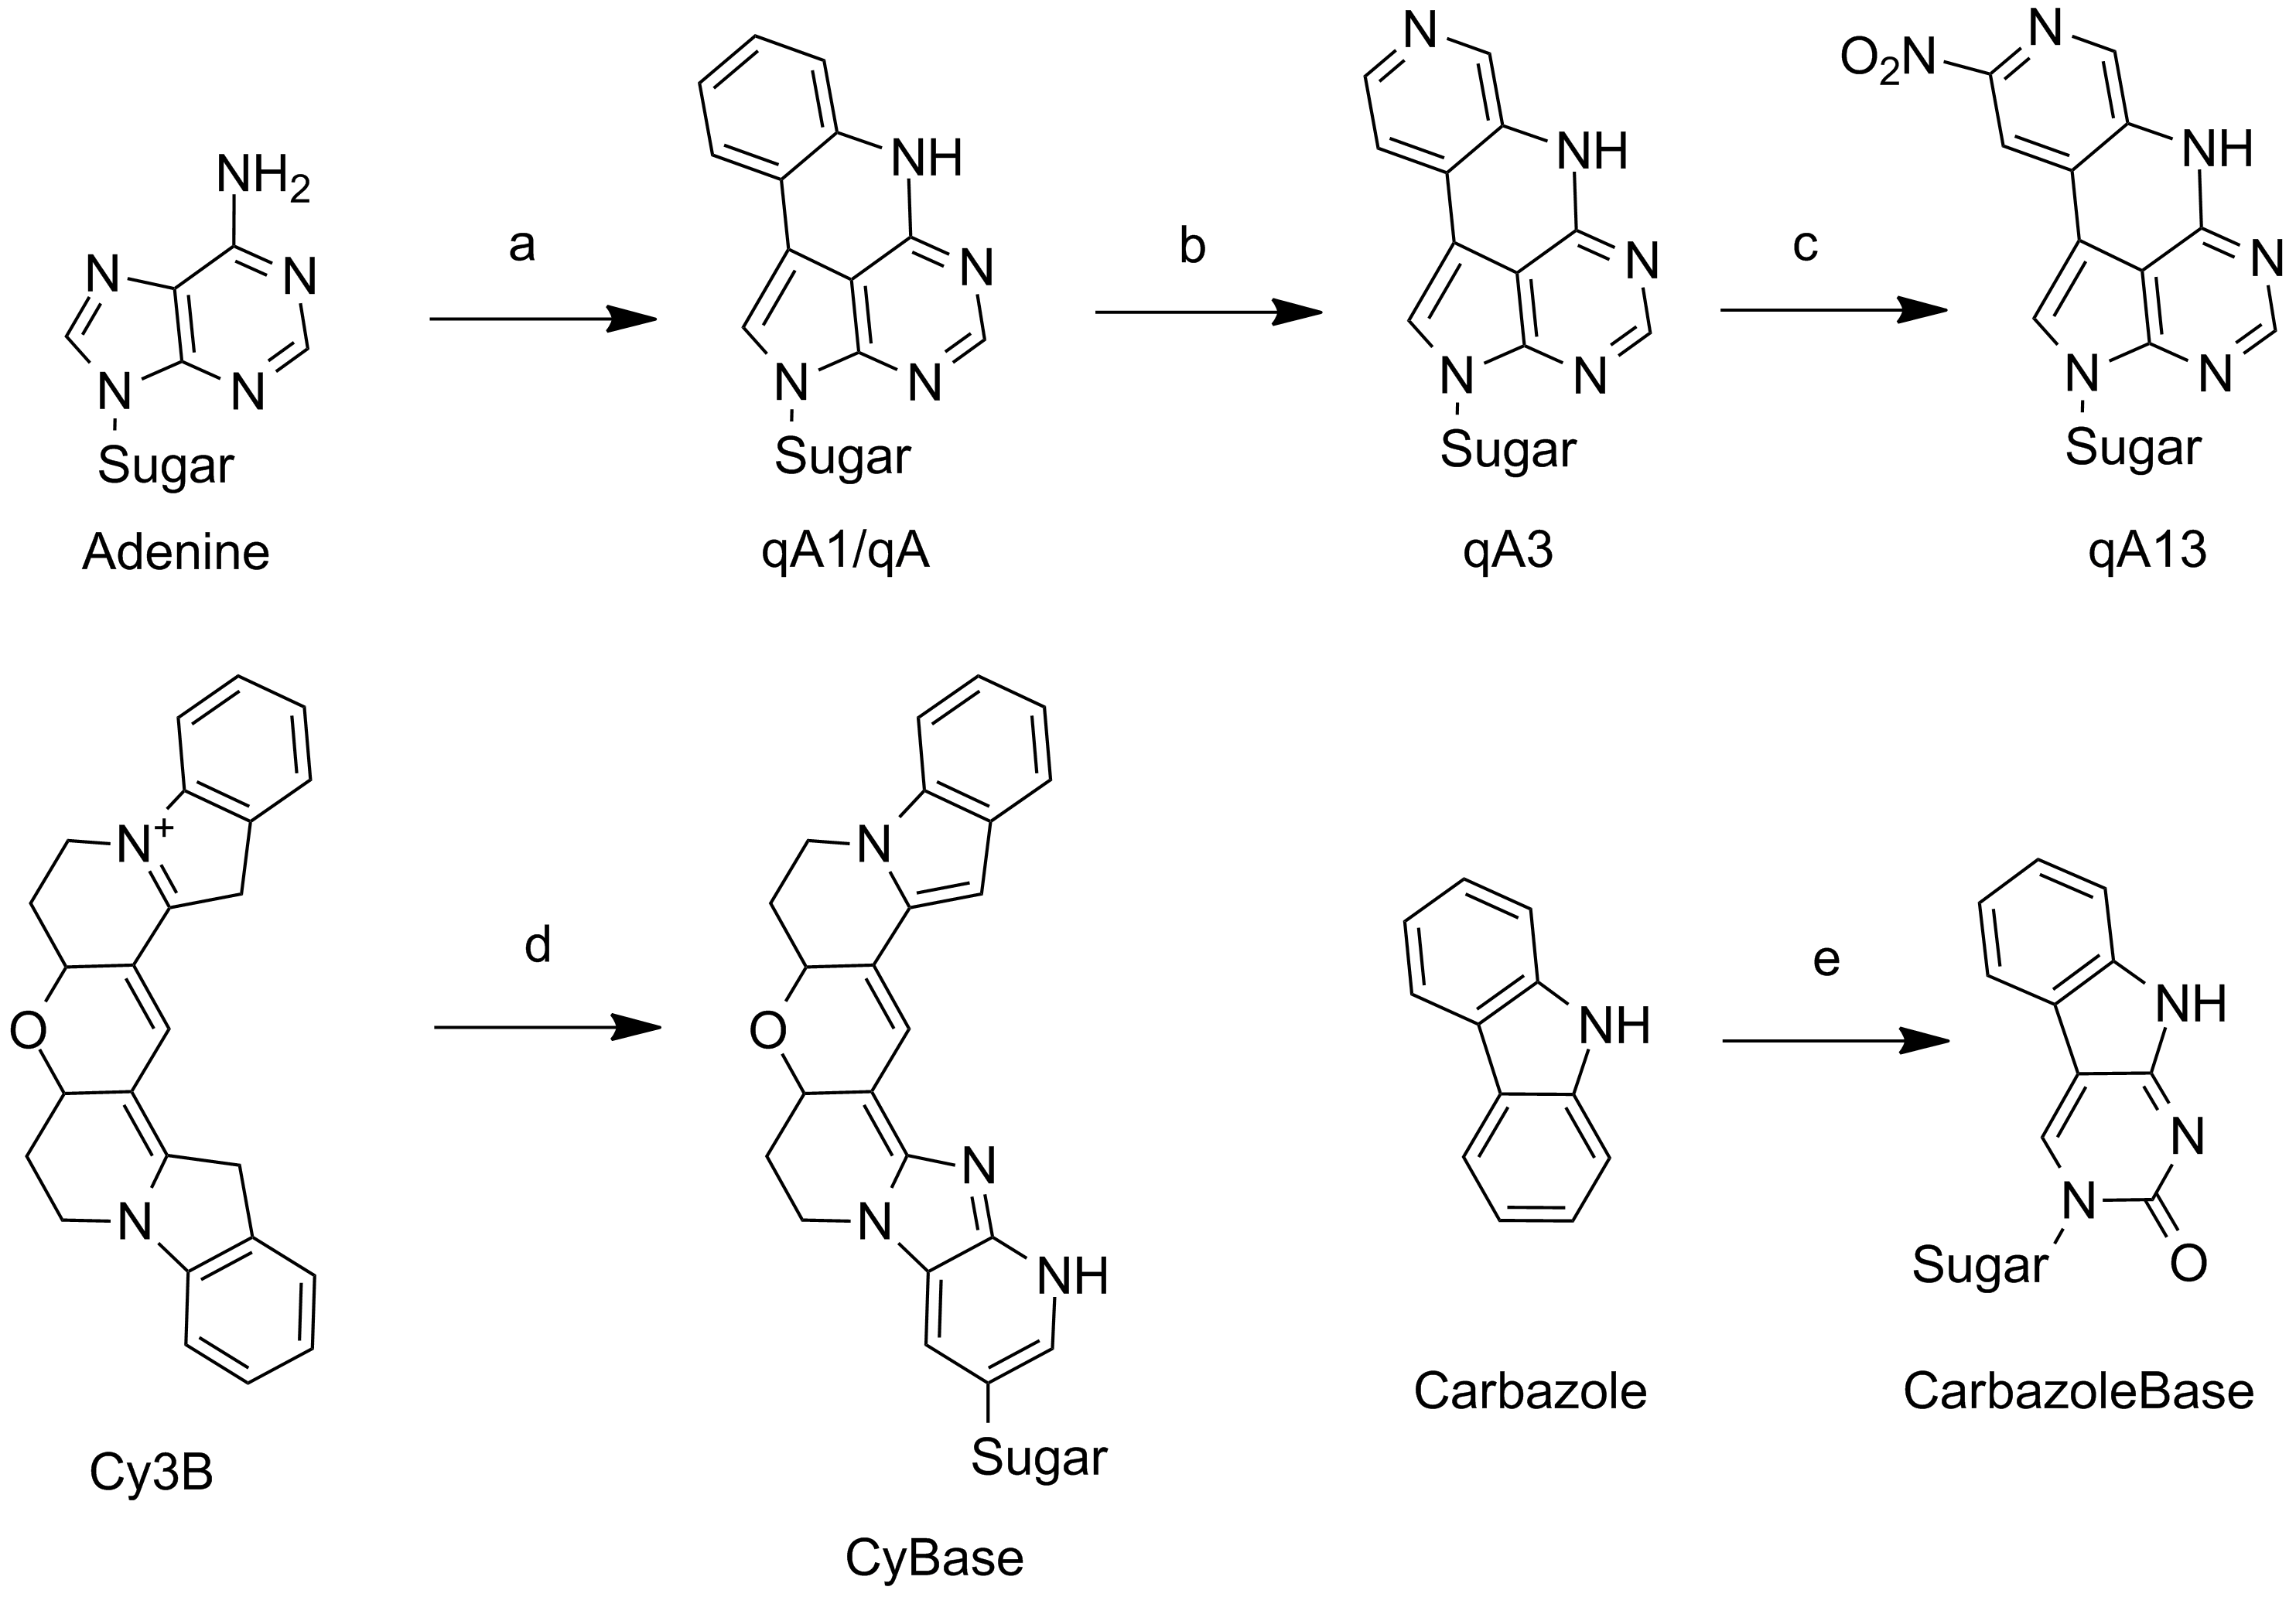
\includegraphics[width=0.95\textwidth]{adds//cej_fig2.png}
    \captionsetup{width=.95\textwidth}
    \caption{Design of fluorescent nucleobase analogues.}
    \label{Fig:chap_Papers_CEJ2}
\end{figure}

 The construction of the base library was achieved from a number of rational considerations and design steps. First, core structures were designed using the canonical bases, adenine, thymine, cytosine and guanine, as starting points. This step is exemplified by qA in Figure \ref{Fig:chap_Papers_CEJ2}a. In the design of the core structures, the goal was to increase the $\pi$-system of the molecule but without causing sterical interactions between the base and its micro environment when positioned in double-stranded DNA, such as interactions with the backbone and neighbouring bases. In addition, the Watson-Crick hydrogen bonding pattern of the bases was maintained. Then, most of the C atoms in the aromatic frameworks of these core structures were systematically substituted by N without affecting the $\pi$-conjugation throughout the molecule (Figure \ref{Fig:chap_Papers_CEJ2}b). Finally, NO$_2$ side-groups were systematically attached to the core structures (Figure \ref{Fig:chap_Papers_CEJ2}c). Aromatic molecules with NO$_2$ side-groups usually cause a red-shifted absorption, as in the case of tC$_\mathrm{nitro}$, which is interesting in the development of novel FRET acceptors. This design strategy resulted in about 90\% of the structures in the library. The other 10\% were designed using known dye structures as starting points functionalized with Watson-Crick hydrogen bonds which includes CyBase based on the Cy3B framework and CarbazoleBase based on the carbazole framework (Figure \ref{Fig:chap_Papers_CEJ2}d and e, respectively).

 It is inherently difficult, practically impossible, to predict all possible excited state decay rate constants of a molecule theoretically, especially in the case where the dye is positioned in demanding environments such as inside the base-stack of double-stranded DNA. This limitation makes it impossible to accurately predict the fluorescence quantum yield or lifetime of a dye that has not yet been synthesized. However, it is possible to increase the probability of a molecular structure to be fluorescent by the combination of different design considerations and predictions. First of all, since fluorescence occurs from the lowest energy electronic transition, S$_1$, the fluorescence rate constant is directly related to the probability of the S$_0$-S$_1$ transition which is reflected in the magnitude of the oscillator strength of this transition.\cite{Strickler1962} Thus, estimating the magnitude of the lowest energy electronic transition theoretically provides a means to estimate the magnitude of the fluorescence rate constant thus increasing the probability that the molecule is fluorescent. However, in order to increase the fluorescence quantum yield the rate of the non-radiative decay pathways must also by minimized. This can be achieved by rigidifying the molecular framework and limiting the number of "floppy" side-groups contributing to the electronic ground and first excited states.\cite{Valeur} In addition, the presence of heavy atoms should be minimized in order to limit intersystem crossing.

 Overall, the most interesting base analogue structures from the library, as seen from a fluorescence application point of view, are identified as those with a lowest energy electronic transition well separated from higher energy transitions, a high oscillator strength of this lowest energy transitions and as red-shifted an excitation energy as possible. The first of these criteria is important in order to use the probe in FRET and fluorescence anisotropy applications since multiple transition dipole moments in the lowest energy absorption band will complicate quantitative data analysis in such experiments. The second criteria is in order to increase the fluorescence rate constant thus increasing the probability of a high fluorescence quantum yield as discussed above. The third criteria is a convenience property since many microscopy setups and laser sources are cheaper and easier to operate for excitation in the visible region of the spectrum and this is thus the standard setup in many laboratories. Furthermore, red-shifted transitions are interesting in the development of FRET acceptors and limits the presence of auto-fluorescence when working with biological samples.

 \paragraph{Most important findings.}Interestingly, the predicted energies and oscillator strengths of the lowest energy electronic transitions of qA were in good agreement with the measured UV-Vis absorption bands of the synthesized probe (Figure \ref{Fig:chap_Papers_CEJ}). The results showed that the lowest energy absorption band of qA contains at least two electronic transitions with the lowest in energy characterized by a relatively small oscillator strength compared to the second lowest in energy. This is an interesting observation because it may explain why qA has a fairly modest fluorescence quantum yield ($\Phi_\mathrm{f} = 6.8\%$) compared to e.g. tC and tC$^\mathrm{O}$: The low fluorescence quantum yield is the result of a low-probability S$_0$-S$_1$ electronic transition "hidden" in the red part of the measured lowest energy absorption band of qA. The predicted directions of the transition dipole moments are also in fairly good agreement with the measured fundamental fluorescence anisotropy excitation spectrum which showed more than one transition hidden in the lowest energy absorption band of qA (Figure 3 in Paper VI).

 Paper VI is an excellent example of how the combination of quantum chemical predictions and rational structure design is extremely powerful in the development of novel fluorophores with predefined properties.

\begin{figure}
    \centering
        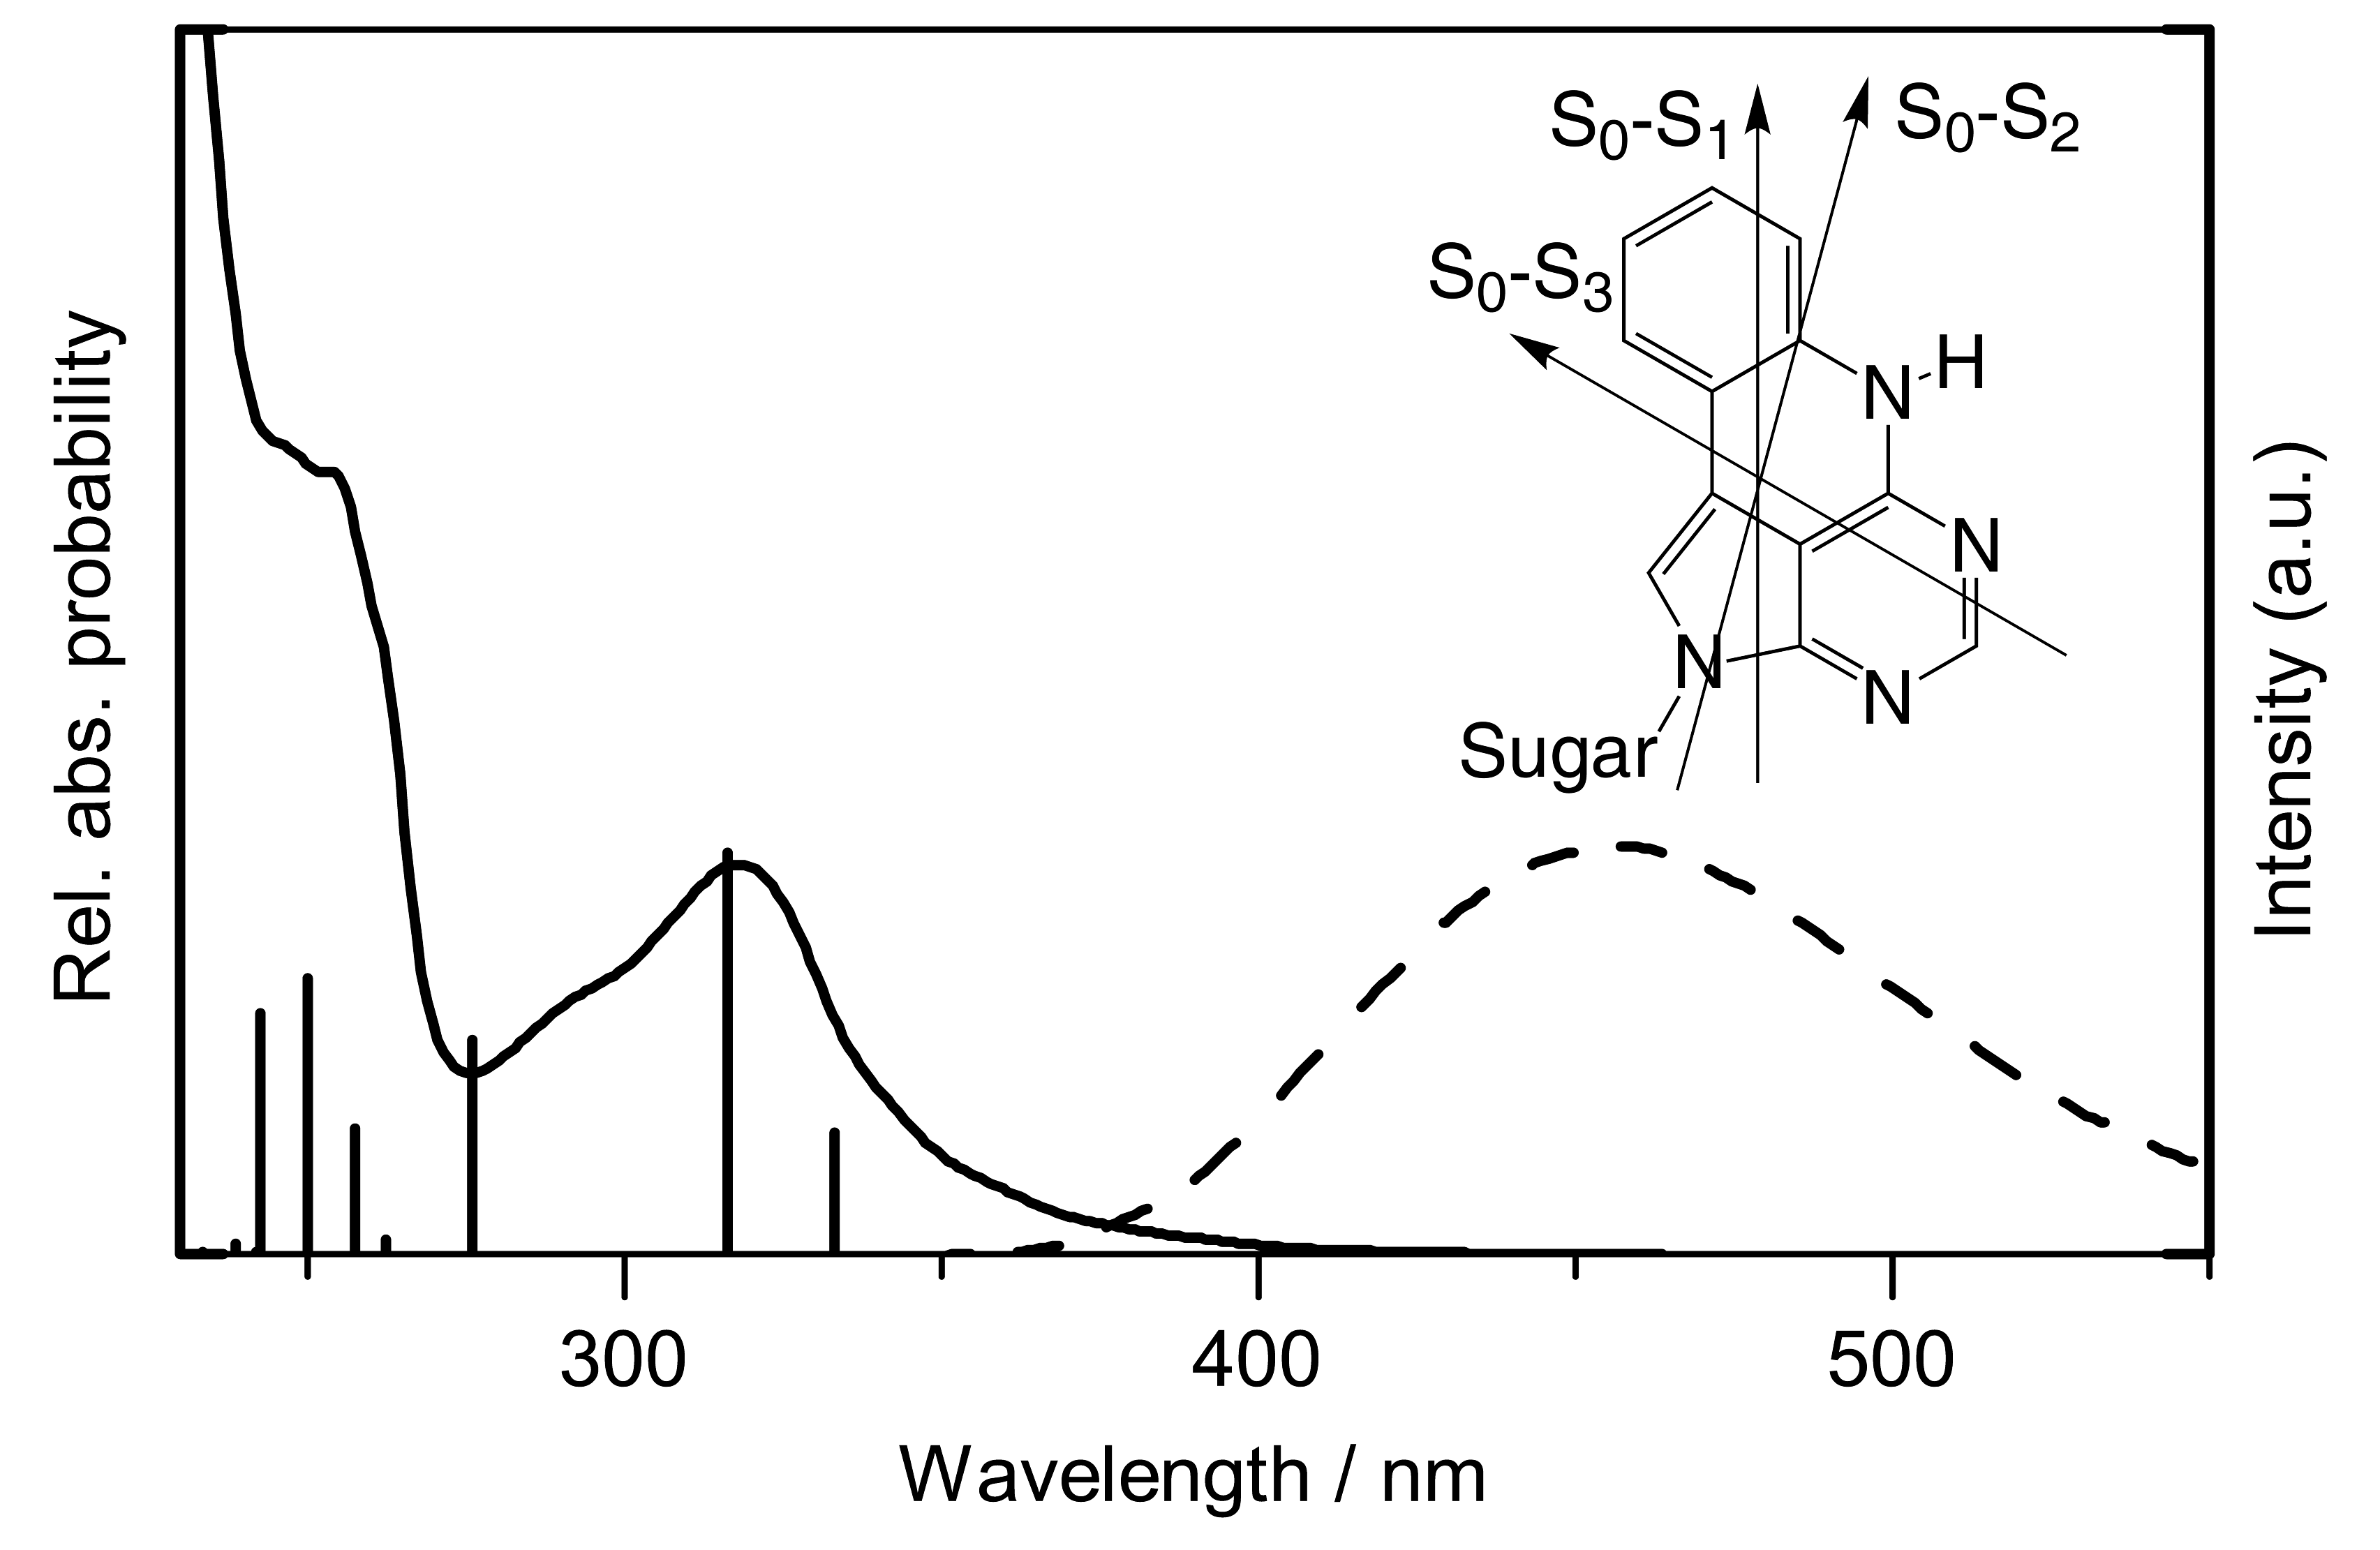
\includegraphics[width=0.6\textwidth]{adds//cej_fig.png}
    \captionsetup{width=.95\textwidth}
    \caption{Predicted lowest energy electronic transitions of qA with measured absorption and emission spectra in H$_2$O.}
    \label{Fig:chap_Papers_CEJ}
\end{figure}


\section{Published Software}
 It is a goal to make the small and larger programs and scripts I develop for myself available to others. All of the programs are written in MATLAB but they are operated through user-interfaces and can be run as stand-alone executables (exe) only requiring a free MATLAB Compiler Runtime (MCR) installed. All the software can be downloaded from:

 \url{www.fluortools.com}

 A comprehensive source of documentation is provided on the home page.

\label{sec_PublishedSoftware}
\subsection{FRETmatrix}
 FRETmatrix is used for the simulation and analysis of base-base FRET (Figure \ref{Fig:chap_Papers_FRETmatrix}). The software has undergone many iterations and a second version that did not make it into the thesis is underway. The theory behind the program is described in Paper III and a User Guide is provided in the Appendix of Paper III. FRETmatrix has since the end of September 2012 been downloaded >20 times from the Chalmers website.
\begin{figure}
    \centering
        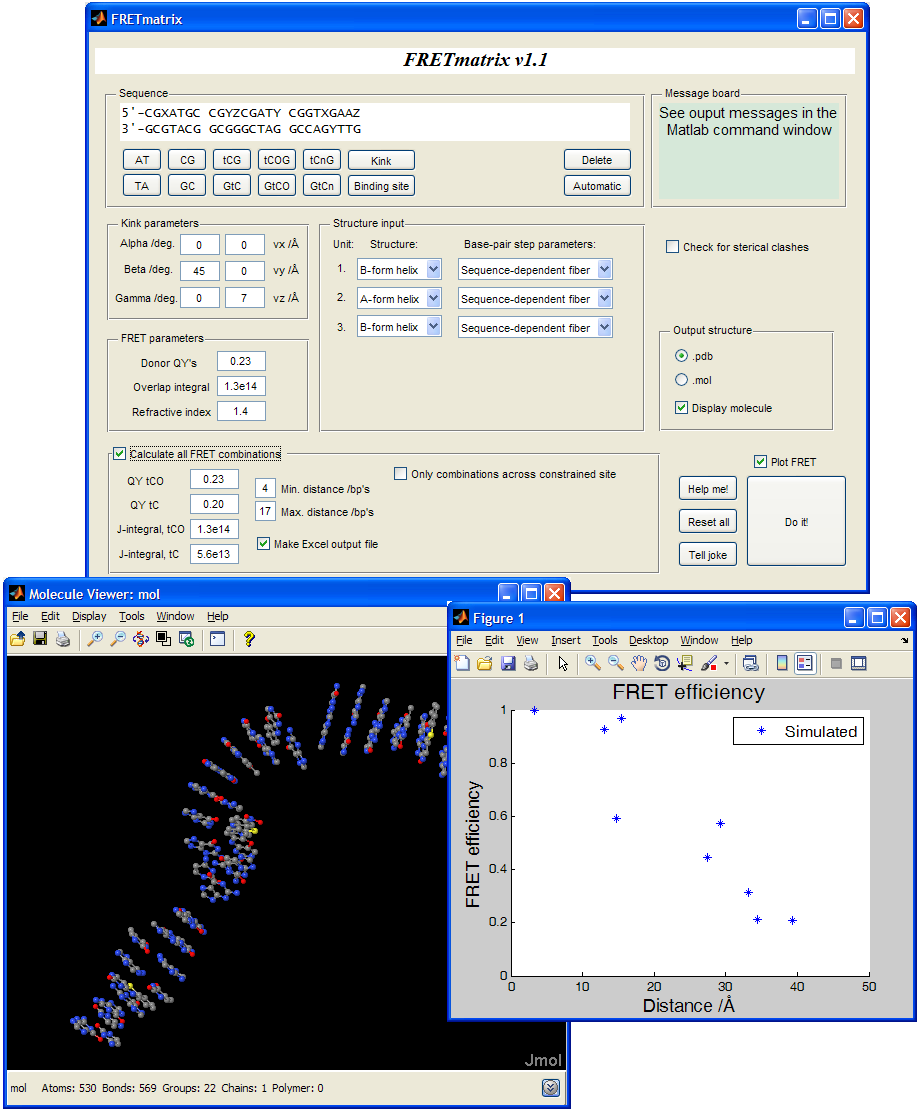
\includegraphics[width=0.95\textwidth]{adds//fretmatrix_fig.png}
    \captionsetup{width=.95\textwidth}
    \caption{Screenshot of FRETmatrix v1.1.}
    \label{Fig:chap_Papers_FRETmatrix}
\end{figure}

\subsection{a|e}
 a|e (pronounced ae) is a software for analyzing, editing and plotting UV-Vis absorption and emission spectra. a|e was made as a free MATLAB-based contrast to commercial data plotting and analysis softwares such as Igor and Origin Pro and is designed particularly for handling and processing multiple UV-Vis spectral datasets simultaneously.

\begin{itemize}
  \item As a spectral analysis software, a|e can be used to calculate fluorescence quantum yields and spectral overlap integrals (for FRET) independent of input data ranges and sizes.
  \item Reference UV-Vis absorption and fluorescence spectra of most commercial dyes can be downloaded directly from Invitrogen's homepage and into a|e for further analysis.
  \item Binding constants or pK$_\mathrm{a}$ values can be obtained from UV-Vis titration measurements by means of singular value decomposition (SVD).
  \item As a spectral editing software a|e can be used to perform mathematical operations to multiple spectra independent of the individual wavelength ranges and stepsizes of the loaded data.
  \item Baselines and light scattering can be subtracted from UV-Vis absorption spectra, the latter \emph{via} a fit to the far-red end of the spectrum (see online documentation page at \url{www.fluortools.com/software/ae/documentation/scatter} for more information).
  \item As with FluorFit and AniFit, the message board can be used as a MATLAB command window for more specialized actions.
  \item For general plotting purposes a|e is meant to handle multiple spectral datasets in a convenient and fast way.
  \item The abscissa is easily alternated in between units of wavelengths (nm) or energy (cm$^{-1}$ or eV).
\end{itemize}

\begin{figure}
    \centering
        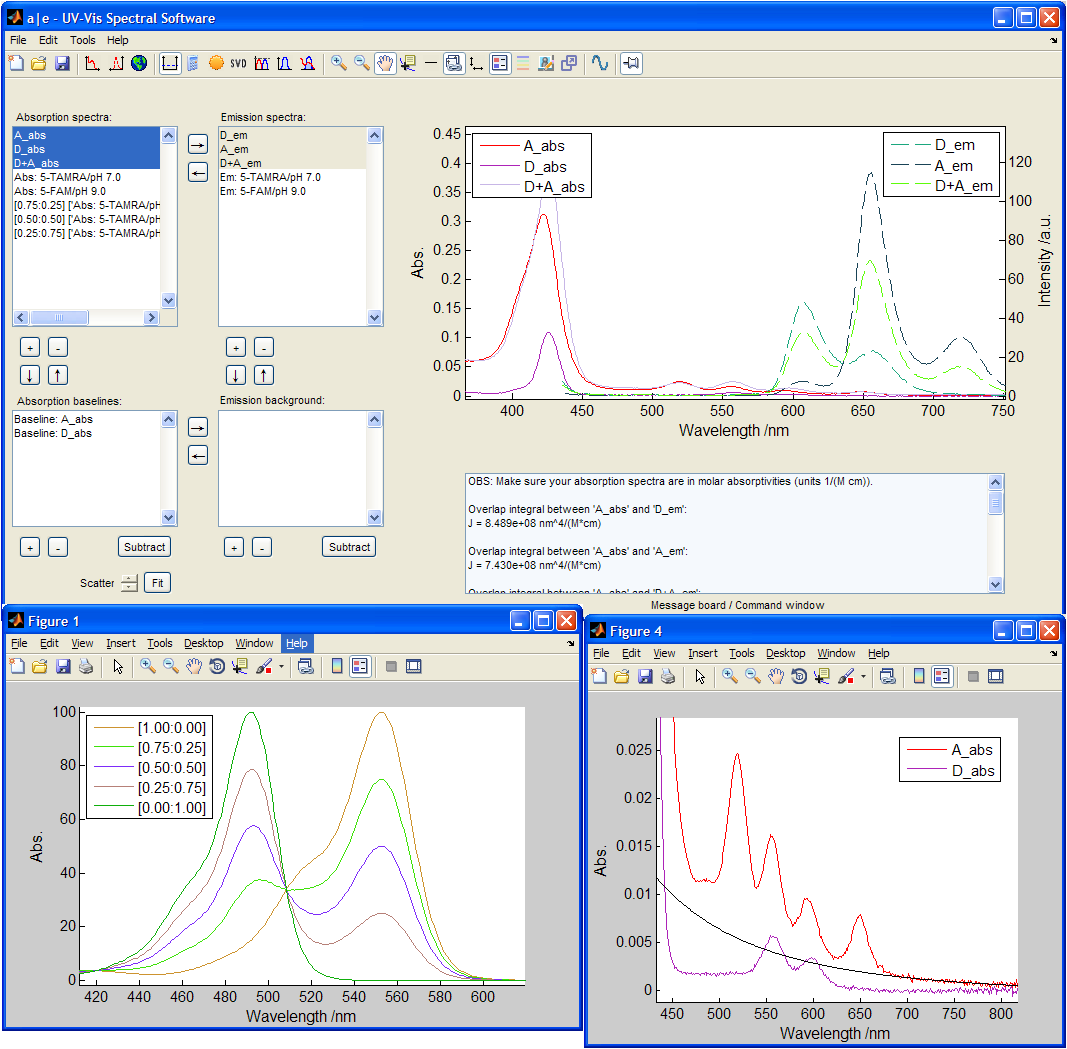
\includegraphics[width=0.95\textwidth]{adds//ae_fig.png}
    \captionsetup{width=.95\textwidth}
    \caption{Screenshot of a|e v1.0.}
    \label{Fig:chap_Papers_ae}
\end{figure}

\subsection{FluorFit}
 FluorFit is a general fluorescence decay fitting software for both standard and more specialized intensity decay analysis (Figure \ref{Fig:chap_Papers_fluorfit}). FluorFit was made because in my experience popular intensity decay reconvolution programs either come with limited features or their license require that they are installed on lab-based computers only. This was inconvenient to me since the lab computer was located in Gothenburg while my office was located in Copenhagen. In addition, using an in-house build software allows for greater flexibility in terms of more specialized and custom data analysis.

\begin{figure}
    \centering
        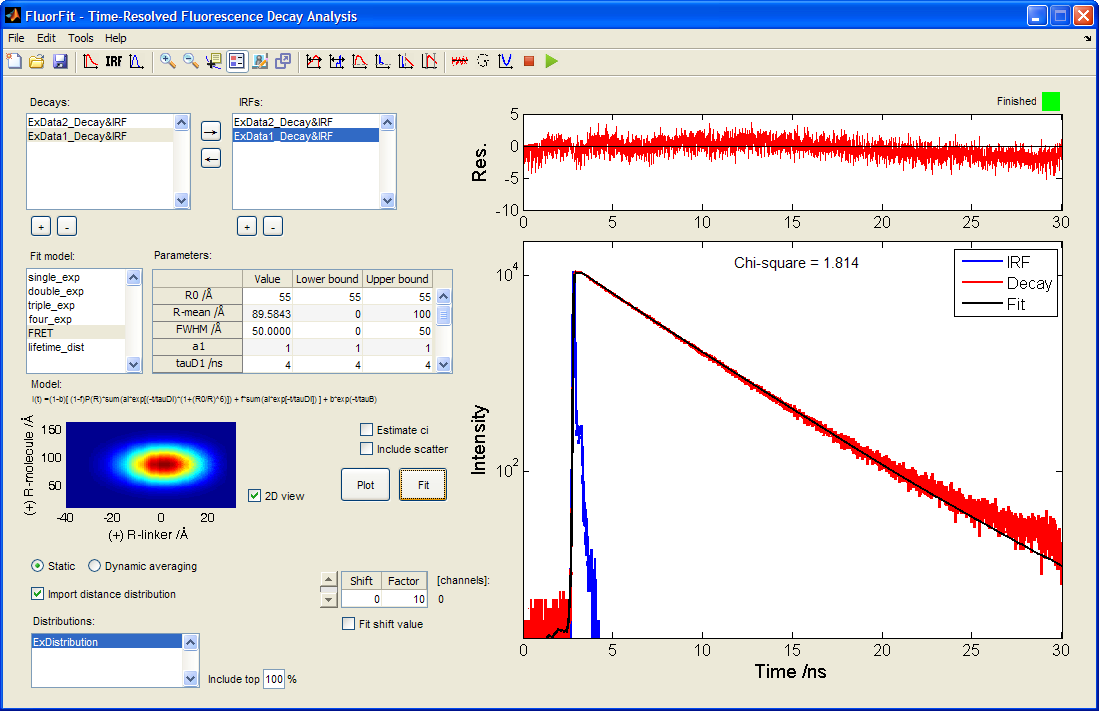
\includegraphics[width=0.95\textwidth]{adds//fluorfit_fig.png}
    \captionsetup{width=.95\textwidth}
    \caption{Screenshot of FluorFit v1.0.}
    \label{Fig:chap_Papers_fluorfit}
\end{figure}

 FluorFit provides most if not all of the fitting features found in commercial programs like Fluofit from PicoQuant and DAS6 from Horiba. FluorFit accepts ASCII-based input files and can handle multiple decays, IRFs and fitting models simultaneously. A FluorFit session can handle multiple graphics window simultaneously and sessions can be saved and reopened. The message board displaying output messages can additionally be used as a MATLAB command window for more specialized actions. Some of the analysis features of FluorFit:
\begin{itemize}
  \item Reconvolution or tailfitting analysis
  \item Imported or user-defined, Gaussian-shaped Instrument Response Functions
  \item Global analysis of multiple decays
  \item Exponential decays or lifetime distributions
  \item FRET analysis using a distribution of donor-acceptor distance: Gaussian or imported distributions
  \item User-defined fitting models
  \item Parameter confidence-interval estimation from the Jacobian matrix
  \item Parameter confidence-interval estimation by calculation of $\chi^2$-surfaces
  \item Autocorrelation plot analysis
  \item Scattering, background and IRF shifting can be taken into account
\end{itemize}

\subsection{AniFit}
\begin{figure}
    \centering
        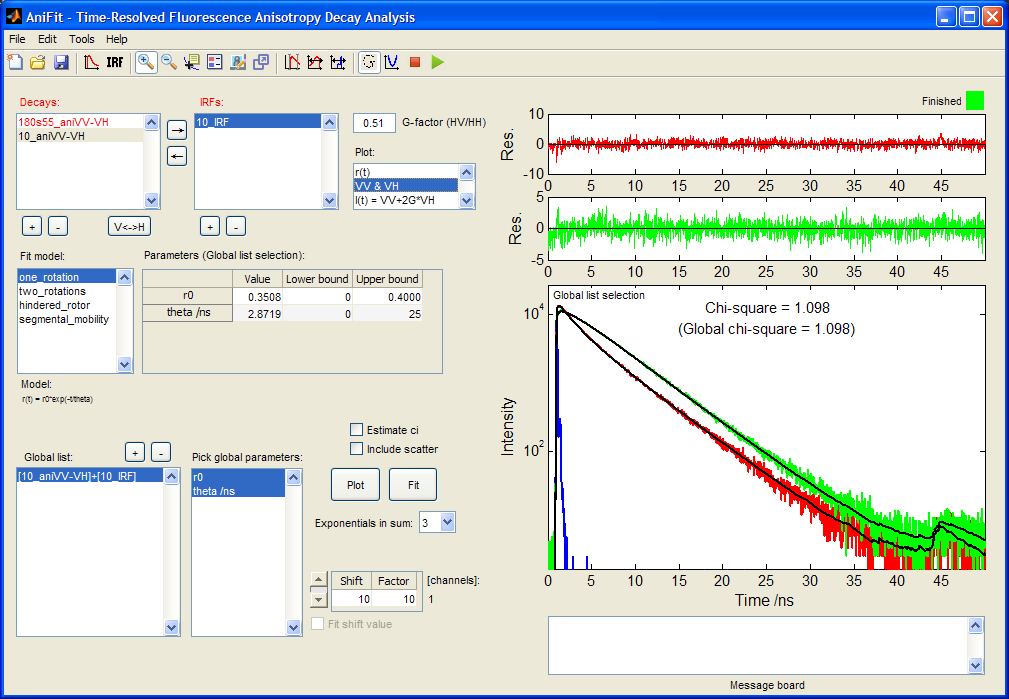
\includegraphics[width=0.95\textwidth]{adds//anifit_fig.png}
    \captionsetup{width=.95\textwidth}
    \caption{Screenshot of AniFit v1.0.}
    \label{Fig:chap_Papers_anifit}
\end{figure}

 AniFit is a time-resolved fluorescence anisotropy decay analysis software (Figure \ref{Fig:chap_Papers_anifit}). AniFit implements a form of global direct vector reconvolution of the vertical and horizontal intensity decay components recorded in an anisotropy experiment in order to optimize the parameters of the anisotropy decay model. First the isotropic fluorophore intensity decay
\[
 I(t) = I_\mathrm{VV} + 2G\times I_\mathrm{VH}
\]
 is optimized using iterative reconvolution with a multiexponential decay. The fitted sum, $I(t)$, is then used as a constraint to simulate each of the $I_\mathrm{VV}$ and $I_\mathrm{VH}$ components:
\[
 I_\mathrm{VV,sim} = \frac{1}{3}I(t)\left[1+2r_\mathrm{model}(t)\right]
\]
\[
 I_\mathrm{VH,sim} = \frac{1}{3}I(t)\left[1-r_\mathrm{model}(t)\right]
\]
 The simulated decays are convolved with the instrument response function:
\[
 I_\mathrm{VV,conv} = \int_{-\infty}^t\mathrm{IRF}(t')\times I_\mathrm{VV,sim}(t-t')dt'
\]
\[
 I_\mathrm{VH,conv} = G\int_{-\infty}^t\mathrm{IRF}(t')\times I_\mathrm{VH,sim}(t-t')dt'
\]
 and iteratively optimized to the measured decays by optimizing the parameter values in the theoretical expression for $r(t)$. This means that AniFit requires a single IRF only (usually VV and VH IRFs are identical).

 AniFit is built on the framework of FluorFit and provides many of the same features listed above but with focus on the analysis of time-resolved fluorescence anisotropy parameters rather than lifetimes.

